% arara: xelatex
% arara: xelatex
% arara: xelatex

% options:
% thesis=B bachelor's thesis
% thesis=M master's thesis
% czech thesis in Czech language
% english thesis in English language
% hidelinks remove colour boxes around hyperlinks

\documentclass[thesis=M,english]{FITthesis}[2019/12/23]

\usepackage[utf8]{inputenc} % LaTeX source encoded as UTF-8

\usepackage{graphicx} %graphics files inclusion
\usepackage{amsmath} %advanced maths
\usepackage{amssymb} %additional math symbols 
\usepackage{mathtools,amscd}

\usepackage{dirtree} %directory tree visualisation
\usepackage{listings}
\usepackage{pdfpages}
\usepackage{float}
\usepackage{svg}

\usepackage{mmacells}
\mmaSet{leftmargin=2em}

% % list of acronyms
% \usepackage[acronym,nonumberlist,toc,numberedsection=autolabel]{glossaries}
% \iflanguage{czech}{\renewcommand*{\acronymname}{Seznam pou{\v z}it{\' y}ch zkratek}}{}
% \makeglossaries

% % % % % % % % % % % % % % % % % % % % % % % % % % % % % % 
% EDIT THIS
% % % % % % % % % % % % % % % % % % % % % % % % % % % % % % 

\department{Department of Information Security}
\title{Multivariate cryptography}
\authorGN{Jan} %author's given name/names
\authorFN{Rahm} %author's surname
\author{Jan Rahm} %author's name without academic degrees
\authorWithDegrees{Bc. Jan Rahm} %author's name with academic degrees
\supervisor{Ing. Jiří Buček, Ph.D.}
\acknowledgements{I would like to thank Ing. Jiří Buček, Ph.D. for the willingness, consultation and valuable advice he gave me.}
\abstractEN{The diploma thesis deals with selected algorithms of multivariate cryptography, especially Unbalanced Oil \& Vintage and Rainbow. The aim of this work is implementation of algorithms in Wolfram Mathematica, investigation of existing solutions and their implementation on ESP32 microcontroller. The algorithms are tested and measured against the RSA and ECDSA algorithms.}
\abstractCS{Diplomová práce se zabývá vybranými algoritmy multivariační kryptografie, zejména Unbalanced Oil \& Vintage a Rainbow. Cílem práce je implementace algoritmů ve Wolfram Mathematica, prozkoumání již existujících řešeních a jejich implementace na mikrokontroleru ESP32. Algoritmy jsou otestovány a změřeny vůči algoritmům RSA a ECDSA.}
\placeForDeclarationOfAuthenticity{Prague}
\keywordsCS{Multivariační kryptografie, Unbalanced Oil \& Vintage, Rainbow, Wolfram Mathematica, ESP32}
\keywordsEN{Multivariate cryptography, Unbalanced Oil \& Vintage, Rainbow, Wolfram Mathematica, ESP32}
\declarationOfAuthenticityOption{1} %select as appropriate, according to the desired license (integer 1-6)
\website{https://github.com/rahmjan/Diploma_Thesis} %optional thesis URL

\begin{document}

% \newacronym{CVUT}{{\v C}VUT}{{\v C}esk{\' e} vysok{\' e} u{\v c}en{\' i} technick{\' e} v Praze}
% \newacronym{FIT}{FIT}{Fakulta informa{\v c}n{\' i}ch technologi{\' i}}

%%%%%%%%%%%%%%%%%%%%%%%%%%%%%%%%%%%%%%%%%%%%
%%%%%%%%%%%%%%%%%%%%%%%%%%%%%%%%%%%%%%%%%%%%
\setsecnumdepth{part}
\chapter{Introduction}
Cryptography is one of the most needed part of modern informatics because almost everyone has something they wish to stay private. But today we can see uprise of the quantum computers which are able to decipher the conventional algorithms for cryptology. That is why a new category of post-quantum cryptography was created and one of its candidates is multivariate cryptography.

The objective of this work is to describe principles of multivariate cryptography for educational purpose with creation of simple example in Wolfram Mathematica. The focus is on Unbalanced Oil \& Vintage and Rainbow algorithms with examination of reference implementation. Further focusing on possible implementation on ESP32 and possible use in IoT.

The final part belongs to comparison with conventional algorithms which are RSA and ECDSA.

%%%%%%%%%%%%%%%%%%%%%%%%%%%%%%%%%%%%%%%%%%%%
%%%%%%%%%%%%%%%%%%%%%%%%%%%%%%%%%%%%%%%%%%%%
\setsecnumdepth{all}
\chapter{Basic terms and definitions}
The chapter describes concepts and algorithms used in the thesis.

\section{Basic terms}
\subsection{Polynomial}
Polynomial $p$ is function to which applies
\[
	p(x) = \sum\limits_{i=0}^n {\alpha_ix^i} = \alpha_0 + \alpha_1x + \alpha_2x^2 + ... + \alpha_nx^n,
\]
where $n \in N_0$ and $\alpha_0, \alpha_1, ..., \alpha_n \in R$. Values $\alpha_0, \alpha_1, ..., \alpha_n$ we calls polynomial coefficients of $p$.  

\subsection{Degree of a polynomial}
The degree of a polynomial is the highest index $i \in N_0$ to which applies that coefficient $\alpha_i \ne 0$. If all coefficients are zero, then the degree of the polynomial is -1.

\subsection{Post-quantum cryptography}
It refers to algorithms that are thought to be secure against an attack by a quantum computer.

But today it is not true for the most used cryptographic algorithms, which are based on mathematical problems of integer factorization, discrete logarithm or elliptic-curve discrete logarithm. These problems can be solved by Shor's algorithm on quantum computer.

\subsection{Finite field}
A finite field is a finite set which is a field. This means that multiplication, addition, subtraction and division (excluding division by zero) are defined and satisfy the rules of arithmetic known as the field axioms.

The simplest examples of finite fields are the fields of prime order: $\mathbb {F}_{p}$ may be constructed as the integers modulo p.

\subsection{Translation}
In Euclidean geometry, a translation is a geometric transformation that moves every point of a figure or a space by the same distance in a given direction.

\subsection{Linear map}
In mathematics, a linear map is a mapping $V \rightarrow W$ between two modules (for example, two vector spaces) that preserves the operations of addition and scalar multiplication.

\subsection{Affine map}
An affine map is the composition of two functions: a translation and a linear map. Ordinary vector algebra uses matrix multiplication to represent linear maps, and vector addition to represent translations. Formally, in the finite-dimensional case, if the linear map is represented as a multiplication by a matrix $A$ and the translation as the addition of a vector $\vec {b}$, an affine map $f$ acting on a vector ${\vec {x}}$ can be represented as:
\[
{\vec {y}}=f({\vec {x}})=A{\vec {x}}+{\vec {b}}
\]

\subsection{Wolfram Mathematica}
Wolfram Mathematica is a computer program widely used in scientific, technical and mathematical circles. The program was originally created by Stephen Wolfram and futher developed by a team of mathematicians and programmers. It is sold by Wolfram Research, with headquartered in Champaign, Illinois.

\subsection{IoT}
Internet of Things (IoT) is a term in computer science for a network of physical devices, vehicles, household appliances, or other devices that are equipped with electronics, software, sensors, moving parts, or network connectivity that allows these devices to connect and exchange data.

\subsection{ESP32}
The ESP32 is a low-cost, low-power microcontroller with integrated Wi-Fi and Bluetooth. It is created and developed by Espressif Systems, a Chinese company based in Shanghai, and is manufactured by TSMC using a 40 nm process.

\bigskip
\noindent
Basic technical parameters are:
\begin{itemize}
\item	CPU: Xtensa dual-core
\item	Memory: 520 KiB SRAM
\item	Wi-Fi: 802.11 b/g/n
\item	Bluetooth: v4.2 BR/EDR and BLE
\item	IEEE 802.11 standard
\item	Hardware acceleration: AES, SHA-2, RSA, ECC, RNG
\end{itemize}

\subsection{RSA}
\subsection{ECDSA}

%%%%%%%%%%%%%%%%%%%%%%%%%%%%%%%%%%%%%%%%%%%%
\newpage
\section{Multivariate cryptography}
\subsection{Definition}
"Multivariate cryptography (MC) is the generic term for asymmetric cryptographic primitives based on multivariate polynomials over a finite field $\mathbb{F}$."\cite{L-WIKI1}

It means it is system of nonlinear polynomial equations with coefficients over a finite filed $\mathbb{F} = \mathbb{F}_q$ with $q$ elements:
\[
	p^{(1)}(x_1,\ldots,x_n) = \sum\limits_{i=1}^{n} {\sum\limits_{j=1}^{n} {p_{ij}^{(1)} \cdot x_ix_j}} + \sum\limits_{i=1}^{n} {p_{i}^{(1)} \cdot x_i} + p_0^{(1)}
\]
\[
	p^{(2)}(x_1,\ldots,x_n) = \sum\limits_{i=1}^{n} {\sum\limits_{j=1}^{n} {p_{ij}^{(2)} \cdot x_ix_j}} + \sum\limits_{i=1}^{n} {p_{i}^{(2)} \cdot x_i} + p_0^{(2)}
\]
\[
	\vdots
\]
\[
	p^{(m)}(x_1,\ldots,x_n) = \sum\limits_{i=1}^{n} {\sum\limits_{j=1}^{n} {p_{ij}^{(m)} \cdot x_ix_j}} + \sum\limits_{i=1}^{n} {p_{i}^{(m)} \cdot x_i} + p_0^{(m)}
\]
 
If the polynomials are of degree two, they are called multivariate quadratics (MQ). Solving systems of multivariate polynomial equations is proven to be NP hard, so called MQ Problem. That is the reason why MC is often considered to be good candidate for post-quantum cryptography.

MC is very fast and requires only moderate computational resources, which makes it attractive for applications in low-cost devices.

\subsection{MQ Problem}
Given $m$ quadratic polynomials $p^{(1)}(x),\ldots,p^{(m)}(x)$ in the $n$ variables $x_1,\ldots,x_n$, find a vector $\bar{x} = (\bar{x}_1,\ldots,\bar{x}_n)$ such that $p^{(1)}(\bar{x}) = \ldots = p^{(m)}(\bar{x}) = 0$.

\subsection{Public key}
The public key of MC is system of MC polynomials. To build this system based on MQ Problem, it needs an easily invertible quadratic map $\mathcal{F}: \mathbb{F}^n \rightarrow \mathbb{F}^m$, so called \textit{central map}. Because it is easily invertible, it needs to be hidden in public key by invertible affine maps: $\mathcal{S}: \mathbb{F}^m \rightarrow \mathbb{F}^m$ and $\mathcal{T}: \mathbb{F}^n \rightarrow \mathbb{F}^n$.

The public key of this system is composed map:
\[
	\mathcal{P} = \mathcal{S} \circ \mathcal{F} \circ \mathcal{T} : \mathbb{F}^n \rightarrow \mathbb{F}^m
\]
and the private key consists of the tree maps $\mathcal{S}$, $\mathcal{F}$ and $\mathcal{T}$, also known as \textit{trapdoor}.

Public key should be hard to invert without the knowledge of the \textit{trapdoor}.

\begin{figure}[h]
\begin{equation*}
  \begin{CD}
     z \in \mathbb{F}^n @>  \mathcal{P} >> w \in \mathbb{F}^m \\
    @V\mathcal{T}VV  @A\mathcal{S}AA \\
  y \in \mathbb{F}^n @> \mathcal{F} >> x \in \mathbb{F}^m
  \end{CD}
\end{equation*}
\caption{Workflow of multivariate public key cryptosystems}
\end{figure}
\smallskip

\subsection{Encryption}
To get a ciphertext $w$, message $z \in \mathbb{F}^n$ can by easily encrypted by evaluation of the public key $\mathcal{P}$:
\[
	w = \mathcal{P}(z) \in \mathbb{F}^m
\]
For decryption of ciphertext, it needs to be evaluated by private key in tree steps: 
\[
	x = \mathcal{S}^{-1}(w) \in \mathbb{F}^m, \, y = \mathcal{F}^{-1}(x) \in \mathbb{F}^n, \, z = \mathcal{T}^{-1}(y) \in \mathbb{F}^n
\]
There is a condition that requires to be $m \geq n$, this way the public key $\mathcal{P}$ will be injective and decryption will output a unique plaintext.

\subsection{Signature}
To generate a signature for a message $m$, it needs to use a hash function:
\[
	\mathcal{H}: \{0,1\}^{*} \rightarrow \mathbb{F}^m
\]
to compute the hash value:
\[
	w = \mathcal{H}(m) \in \mathbb{F}^m
\]
After this step it can be evaluated by:
\[
	x = \mathcal{S}^{-1}(w) \in \mathbb{F}^m, \, y = \mathcal{F}^{-1}(x) \in \mathbb{F}^n, \, z = \mathcal{T}^{-1}(y) \in \mathbb{F}^n
\]
where $z$ is the signature of message $m$. As can be seen, it is similar to description of ciphertext.

The verification of signature $z$ is done by computing the hash value:
\[
	w = \mathcal{H}(m) \in \mathbb{F}^m
\]
and by evaluation of public key $\mathcal{P}$:
\[
	w' = \mathcal{P}(z) \in \mathbb{F}^m
\]
If $w' = w$ is true, the signature is valid, otherwise not.

There is also condition that requires to be $m \leq n$, this way the public key $\mathcal{P}$ will be surjective and private key can sign any message.

%%%%%%%%%%%%%%%%%%%%%%%%%%%%%%%%%%%%%%%%%%%%
\section{UOV}
The Unbalanced Oil and Vinegar's name comes from the fact that the variables of the polynomials are grouped into two groups: the vinegar and the oil. These two groups are mixed in the polynomials and the unbalanced attribute refers to the ratio of the variables, where is always more vinegar than oil variables. The signature scheme was proposed by Kipnis and Patarin in 1999.

\subsection{Definition}
Let $\mathbb{F}$ be a finite field, $v,o \in \mathbb{N}$ and $n=v+o$, $V=\{1, \ldots, v\}$, $O=\{v+1, \ldots, n\}$. The variables $x_1, \ldots, x_v$ are Vinegar variables and $x_{v+1}, \ldots, x_n$ are Oil variables. If $v=o$ the scheme is called balanced Oil \& Vinegar (OV), for $v>o$ it is UOV.

\bigskip
\noindent
The \textit{central map} $\mathcal{F}:\mathbb{F}^n \rightarrow \mathbb{F}^o$ consist of $o$ quadratic polynomials $f^{(1)}, \ldots, f^{(o)}$:
\[
	f^{(k)} = \sum\limits_{i=1}^{v} {\sum\limits_{j=1}^{v} {\alpha_{ij}^{(k)} \cdot x_ix_j}} +  \sum\limits_{i=1}^{v} {\sum\limits_{j=v+1}^{n} {\beta_{ij}^{(k)} \cdot x_ix_j}}+ \sum\limits_{i=1}^{n} {\gamma_{i}^{(k)} \cdot x_i} + \delta^{(k)}
\]
where $\alpha_{ij}^{(k)}$, $\beta_{ij}^{(k)}$, $\gamma_{i}^{(k)}$, $\delta^{(k)} \in \mathbb{F}$ and $1 \leq k \leq o$.

\bigskip
\noindent
To hide $\mathcal{F}$ in the public key, it is combined with one invertible affine map $\mathcal{T}: \mathbb{F}^n \rightarrow \mathbb{F}^n$. The public key of the scheme is in the form:
\[
	\mathcal{P} = \mathcal{F} \circ \mathcal{T} : \mathbb{F}^n \rightarrow \mathbb{F}^o
\]
and the private key consist of $\mathcal{F}$ and $\mathcal{T}$. The second affine map $\mathcal{S}$ is not needed for the security of UOV.

\subsection{Security}
For the security of UOV is required $v \geq 2o$ because of the attack of Kipnis and Shamir on balanced OV.\cite{L-KS98} Besides of that, the UOV scheme resisted (for suitable parameter sets) cryptanalysis for over 20 years. Now it is one of the oldest and best studied cryptosystems and is therefore believed to be of high security.

The UOV scheme is very simple, has small signatures and is fast. The main disadvantage is its public keys which are quite large.

%%%%%%%%%%%%%%%%%%%%%%%%%%%%%%%%%%%%%%%%%%%%
\newpage
\section{Rainbow}
The Rainbow is a multi layer version of UOV. The layers are not independent from each other but there is a hierarchy which uses the results from the layer above to compute additional variables. The name comes from the link to the layers of a rainbow and the scheme was introduced by Ding and Schmid in 2005.

The main advantage compared to UOV should be in better performance, smaller key sizes and smaller signatures.

\subsection{Definition}
Let $\mathbb{F}$ be a finite field, $0<v_1<v_2<\ldots<v_{u+1} = n$ be a sequence of integers and $V_i=\{1, \ldots, v_i\}$, $O_i=\{v_i+1, \ldots, v_{i+1}\}$ and $o_i = v_{i+1} - v_i \,\, (i=1,\ldots,u)$ where $o_i$ is number of oil variables and $u$ is number of UOV instances.

\bigskip
\noindent
The \textit{central map} $\mathcal{F}:\mathbb{F}^n \rightarrow \mathbb{F}^m$ consist of $m = n - v_1$ quadratic polynomials $f^{(v_1+1)}, \ldots, f^{(n)}$:
\[
	f^{(k)} = \sum\limits_{i,j \in V_l}{\alpha_{ij}^{(k)} \cdot x_ix_j} +  \sum\limits_{i \in V_l,j \in O_l}{\beta_{ij}^{(k)} \cdot x_ix_j}+ \sum\limits_{i \in V_l \cup O_l}{\gamma_{i}^{(k)} \cdot x_i} + \delta^{(k)}
\]
where $l \in \{1, \ldots, u\}$ is the only integer such that $k \in O_l$ and $\alpha_{ij}^{(k)}$, $\beta_{ij}^{(k)}$, $\gamma_{i}^{(k)}$, $\delta^{(k)} \in \mathbb{F}$.

\bigskip
\noindent
To hide $\mathcal{F}$ in the public key, it is combined with two invertible affine maps $\mathcal{T}: \mathbb{F}^n \rightarrow \mathbb{F}^n$ and $\mathcal{S}: \mathbb{F}^m \rightarrow \mathbb{F}^m$. The public key of the scheme is in the form:
\[
	\mathcal{P} = \mathcal{S} \circ \mathcal{F} \circ \mathcal{T} : \mathbb{F}^n \rightarrow \mathbb{F}^m
\]
and the private key consist of $\mathcal{S}$, $\mathcal{F}$ and $\mathcal{T}$.

%%%%%%%%%%%%%%%%%%%%%%%%%%%%%%%%%%%%%%%%%%%%
%%%%%%%%%%%%%%%%%%%%%%%%%%%%%%%%%%%%%%%%%%%%
\chapter{Realization}
Chapter describes implementation of algorithms on selected platforms which are Wolfram Mathematica, PC and microcontroller ESP32. For the last two specified the implementation is in language C++.

\section{Wolfram Mathematica}
This section describes examples in Wolfram Mathematica and step by step description of algorithms.

\subsection{UOV}
Here is description of signature scheme of UOV. This example of UOV is in fact example of balanced OV because it simplify the explanation of the algorithm.

\bigskip
\noindent
First set up the parameters of the example: 
Let $\mathbb{F} = GF(7)$, $o=v=3$. The central map $\mathcal{F} = (f^{(1)}, f^{(2)}, f^{(3)})$ is given by:
\begin{mmaCell}[addtoindex=2,moredefined={mod, F1, F2, F3},morepattern={x1_, x2_, x3_, x4_, x5_, x6_, x1, x2, x3, x4, x5, x6}]{Input}
  mod=7;
  F1[x1_,x2_,x3_,x4_,x5_,x6_]:=
4x1^2+4x1*x3+5x1*x4+6x1*x5+x1*x6+6x1+4x2^2+x2*x3+6x2*x4
+6x2*x5+5x2*x6+5x2+5x3^2+3x3*x4+5x3*x5+2x3*x6+5x3+6x4+3x5;
  F2[x1_,x2_,x3_,x4_,x5_,x6_]:=
3x1*x3+4x1*x4+3x1*x5+4x1*x6+3x1+6x2^2+x2*x3+4x2*x4+4x2*x5
+5x2*x6+6x2+6x3^2+4x3*x4+2x3*x5+x3*x6+3x3+x4+x6+1;
  F3[x1_,x2_,x3_,x4_,x5_,x6_]:=
6x1^2+6x1*x3+4x1*x5+2x1*x6+2x2^2+5x2*x3+6x2*x4+5x2*x5+
5x2*x6+6x2+3x3^2+5x3*x4+6x3*x5+x3*x6+3x3+4x4+6x5+5;
\end{mmaCell}
It will set up the value of $mod$ to 7 and initialize functions of the central map. Next is setting up of the affine map $\mathcal{T}$ with matrix $A$ and vector $b$. These two parts will be later used separately in the example. 
\begin{figure}[h]
	\begin{minipage}{0.42\textwidth}
		\centering
		\begin{mmaCell}[addtoindex=3,moredefined={A}]{Input}
  A=(6 5 5 5 5 4
     6 6 4 5 0 6
     2 5 2 1 5 0
     1 1 6 2 2 3
     3 6 2 2 3 0
     0 5 4 6 1 5);
		\end{mmaCell}
	\end{minipage}
	\begin{minipage}{0.28\textwidth}
		\centering
		\begin{mmaCell}[moredefined={b}]{Input}
  b=(1
     2
     4
     1
     3
     2);
		\end{mmaCell}
	\end{minipage}
	\begin{minipage}{0.2\textwidth}
		\centering
		\begin{mmaCell}[moredefined={T, A, b}]{Input}
  T=A.(x1
       x2
       x3
       x4
       x5
       x6)+b; 
		\end{mmaCell}
	\end{minipage}
\end{figure}

\noindent
This block computes public key $\mathcal{P}$ by putting values of $\mathcal{T}$ inside of $\mathcal{F}$, it also simplify the expression of $p1,p2,p3$ and finally applies modulo on whole polynomial:
\begin{mmaCell}[moredefined={p1, F1, T, p2, F2, p3, F3, P1, mod, P2, P3},morepattern={x1_, x2_, x3_, x4_, x5_, x6_}]{Input}
  p1 = F1 @@ T[[All]];
  p2 = F2 @@ T[[All]];
  p3 = F3 @@ T[[All]];
  P1[x1_,x2_,x3_,x4_,x5_,x6_] = PolynomialMod[Simplify[p1],mod]
  P2[x1_,x2_,x3_,x4_,x5_,x6_] = PolynomialMod[Simplify[p2],mod]
  P3[x1_,x2_,x3_,x4_,x5_,x6_] = PolynomialMod[Simplify[p3],mod]
\end{mmaCell}

\noindent
The results of $\mathcal{P} = \mathcal{F} \circ \mathcal{T}$ are:
\begin{mmaCell}[addtoindex=3]{Output}
  \{6+x1+5x2+4x1x2+2\mmaSup{x2}{2}+3x3+x1x3+x2x3+\mmaSup{x3}{2}+6x4+2x1x4+5x2x4+2x3x4
+3\mmaSup{x4}{2}+5x5+3x1x5+6x2x5+4x3x5+3x4x5+4\mmaSup{x5}{2}+4x6+x2x6+3x3x6+2x4x6\}
\end{mmaCell}
\begin{mmaCell}{Output}
  \{5+6\mmaSup{x1}{2}+5x2+4x1x2+5\mmaSup{x2}{2}+4x3+5x1x3+3x2x3+2\mmaSup{x3}{2}+2x4+2x1x4+4x2x4
+2x3x4+5\mmaSup{x4}{2}+3x5+5x1x5+5x2x5+2x3x5+6\mmaSup{x5}{2}+5x2x6+6x4x6+2x5x6+6\mmaSup{x6}{2}\}
\end{mmaCell}
\begin{mmaCell}{Output}
  \{5+5x1+4\mmaSup{x1}{2}+5x2+3x1x2+5\mmaSup{x2}{2}+2x3+2x1x3+x2x3+2\mmaSup{x3}{2}+6x4+3x2x4+2\mmaSup{x4}{2}
+x5+3x1x5+6x2x5+4x3x5+2\mmaSup{x5}{2}+2x6+x1x6+3x2x6+4x3x6+6x4x6+5x5x6+4\mmaSup{x6}{2}\}
\end{mmaCell}
From this place on it will only focus on computation of signature $z$ for message $w$. Be aware that in this example is not used hash function for the message because for the example purpose it is not needed.
\begin{mmaCell}[moredefined={w, y1, y2, y3}]{Input}
  w  = \{\{3\},\{6\},\{4\}\};
  y1 = 1;
  y2 = 0;
  y3 = 6;
\end{mmaCell}
It sets the message to value $w = (3,6,4)$ and also it set values for $y = (y1,y2,y3)$. These values for $y$ are randomly chosen.
\begin{mmaCell}[addtoindex=3,moredefined={f1, F1, y1, y2, y3, mod, f2, F2, f3, F3}]{Input}
  f1 = PolynomialMod[F1[y1,y2,y3,y4,y5,y6],mod]
  f2 = PolynomialMod[F2[y1,y2,y3,y4,y5,y6],mod]
  f3 = PolynomialMod[F3[y1,y2,y3,y4,y5,y6],mod]
\end{mmaCell}
Here are the results after minimalizing and use of modulo:
\begin{mmaCell}{Output}
  f1 = 6+y4+4y5+6y6
  f2 = 4+y4+y5+4y6
  f3 = 5+6y4+4y5+y6
\end{mmaCell}
Next two steps solve linear system $f^{(1)} = w_1 = 3, f^{(2)} = w_2 = 6, f^{(3)} = w_3 = 4$, it can also use for the solution the Gaussian elimination:
\begin{mmaCell}[moredefined={res, f1, w, f2, f3, mod}]{Input}
  res = Solve[\{f1==w[[1]], f2==w[[2]], f3==w[[3]]\},Modulus \(\pmb{\to}\) mod];
\end{mmaCell}
\begin{mmaCell}[moredefined={y, y1, y2, y3, res}]{Input}
  y = \{y1,y2,y3,y4,y5,y6\} /. res 
\end{mmaCell}
\begin{mmaCell}{Output}
  \{\{1,0,6,6,3,0\}\}
\end{mmaCell}
It will obtain results for $(y4,y5,y6) = (6,3,0)$. After combination it is $y = (1,0,6,6,3,0)$, so called \textit{pre-image} of $w$: $y =  \mathcal{F}^{-1}(w)$. If the solution for linear system do not exist, choose different values for $(y1,y2,y3)$ and repeat steps before.

\bigskip
\noindent
Finally use $\mathcal{T}^{-1}$ to compute signature $z$. For that is needed inversion of matrix $A$.
\begin{figure}[h]
	\begin{minipage}{0.59\textwidth}
		\centering
\begin{mmaCell}[moredefined={A, mod}]{Input}
  \mmaSub{A}{-1} = Inverse[A, Modulus\(\pmb{\to}\)mod]
\end{mmaCell}
	\end{minipage}
	\begin{minipage}{0.28\textwidth}
		\centering
		\begin{equation*}
A_{-1} = 
\begin{pmatrix}
2 & 4 & 6 & 2 & 0 & 5 \\
1 & 3 & 3 & 1 & 6 & 2 \\
4 & 6 & 6 & 4 & 5 & 4 \\
2 & 0 & 3 & 4 & 2 & 3 \\
6 & 0 & 3 & 0 & 0 & 5 \\
2 & 2 & 2 & 5 & 3 & 3
\end{pmatrix}
\end{equation*}
	\end{minipage}
\end{figure}
\begin{mmaCell}[moredefined={z, A, y, b, mod}]{Input}
  z = Mod[\mmaSub{A}{-1}.(Transpose[y]-b),mod] 
\end{mmaCell}
\begin{mmaCell}{Output}
  \{\{4\},\{1\},\{5\},\{6\},\{3\},\{5\}\}
\end{mmaCell}
The value of the signature $z = (4,1,5,6,3,5)$.

\bigskip
\noindent
Last part is check if two hashes (in this example two messages $w$) are the same.
\begin{mmaCell}[moredefined={w2, w, P1, z, P2, P3, mod}]{Input}
  w2=w;
  w2=\{P1 @@ z[[All,1]],P2 @@ z[[All,1]],P3 @@ z[[All,1]]\};
  (* True? *)
  Mod[w2,mod]==w
\end{mmaCell}
\begin{mmaCell}[addtoindex=2]{Output}
  True
\end{mmaCell}

The file with implementation can by find under name "UOV.nb".

%%%%%%%%%%%%%%%%%%%
\subsection{Rainbow}
The description of signature scheme of Rainbow is very similar to the description of OV.

\bigskip
\noindent
First set up the parameters of the example: 
Let $\mathbb{F} = GF(7)$, $v1=o1=o2=2$. The central map $\mathcal{F} = (f^{(3)}, f^{(4)}, f^{(5)}, f^{(6)})$ is given by:
\begin{mmaCell}[addtoindex=2,moredefined={mod, F3, F4, F5, F6},morepattern={x1_, x2_, x3_, x4_, x5_, x6_, x1, x2, x3, x4, x5, x6}]{Input}
  mod=7;
  F3[x1_,x2_,x3_,x4_,x5_,x6_]:= 
x1^2+3x1*x2+5x1*x3+6x1*x4+2x2^2+6x2*x3+4x2*x4+2x2+6x3+2x4+5;
  F4[x1_,x2_,x3_,x4_,x5_,x6_]:= 
2x1^2+x1*x2+x1*x3+3x1*x4+4x1+x2^2+x2*x3+4x2*x4+6x2+x4;
  F5[x1_,x2_,x3_,x4_,x5_,x6_]:= 
2x1^2+3x1*x2+3x1*x3+3x1*x4+x1*x5+3x1*x6+6x1+4x2^2+x2*x3+
4x2*x4+x2*x5+3x2*x6+3x2+3x3*x4+x3*x5+2x3*x6+2x3+3x4*x5+x5+6x6;
  F6[x1_,x2_,x3_,x4_,x5_,x6_]:= 
2x1^2+5x1*x2+x1*x3+5x1*x4+5x1*x6+6x1+5x2^2+3x2*x3+5x2*x5+4x2*x6
+x2+3x3^2+5x3*x4+4x3*x5+2x3*x6+4x3+x4^2+6x4*x5+3x4*x6+4x4+4x5+x6+2;
\end{mmaCell}
Next is setting up of the affine map $\mathcal{T}$ with matrix $A$ and vector $b$ which are the same as in OV example. But with addition of affine map $\mathcal{S}$ with matrix $A2$ and vector $b2$.
\begin{figure}[H]
	\begin{minipage}{0.39\textwidth}
		\centering
		\begin{mmaCell}[addtoindex=3,moredefined={A2}]{Input}
  A2=(6 5 5 5
      6 6 4 5
      2 5 2 1
      1 1 6 2);
		\end{mmaCell}
	\end{minipage}
	\begin{minipage}{0.3\textwidth}
		\centering
		\begin{mmaCell}[moredefined={b2}]{Input}
  b2=(1
      2
      4
      1);
		\end{mmaCell}
	\end{minipage}
	\begin{minipage}{0.2\textwidth}
		\centering
		\begin{mmaCell}[moredefined={S, A2, b2}]{Input}
  S=A2.(x1
        x2
        x3
        x4)+b2; 
		\end{mmaCell}
	\end{minipage}
\end{figure}

\noindent
This block computes public key $\mathcal{P}$ by putting values of $\mathcal{T}$ inside of $\mathcal{F}$ and after it makes from matrix S functions which are used for final step of computation of $\mathcal{P}$, it also simplify the expression of $pp3,pp4,pp5,pp6$ and finally applies modulo on whole polynomial:
\begin{mmaCell}[moredefined={p3, p4, p5, p6, S3, S4, S5, S6, mod, P3, P4, P5, P6, pp3,pp4,pp5,pp6, F3, F4, F5,F6, T, S},morepattern={x1_, x2_, x3_, x4_, x5_, x6_}]{Input}
p3 = F3 @@ T[[All]];
p4 = F4 @@ T[[All]];
p5 = F5 @@ T[[All]];
p6 = F6 @@ T[[All]];
S3[x1_,x2_,x3_,x4_] = S[[1]];
S4[x1_,x2_,x3_,x4_] = S[[2]];
S5[x1_,x2_,x3_,x4_] = S[[3]];
S6[x1_,x2_,x3_,x4_] = S[[4]];
pp3 = S3[p3,p4,p5,p6][[1]];
pp4 = S4[p3,p4,p5,p6][[1]];
pp5 = S5[p3,p4,p5,p6][[1]];
pp6 = S6[p3,p4,p5,p6][[1]];
P3[x1_,x2_,x3_,x4_,x5_,x6_] = PolynomialMod[Simplify[pp3],mod];
P4[x1_,x2_,x3_,x4_,x5_,x6_] = PolynomialMod[Simplify[pp4],mod];
P5[x1_,x2_,x3_,x4_,x5_,x6_] = PolynomialMod[Simplify[pp5],mod];
P6[x1_,x2_,x3_,x4_,x5_,x6_] = PolynomialMod[Simplify[pp6],mod];
\end{mmaCell}

\noindent
Computation $x$ from message $w$: $x = \mathcal{T}^{-1}(w)$ :
\begin{mmaCell}[moredefined={w, A2, b2, S, x, mod}]{Input}
w = \{\{2\},\{2\},\{3\},\{4\}\};
\mmaSub{A2}{-1} = Inverse[A2, Modulus\(\pmb{\to}\)mod]
x = Mod[\mmaSub{A2}{-1}.(w - b2),mod]
\end{mmaCell}
\begin{mmaCell}{Output}
  \{\{6\},\{0\},\{1\},\{6\}\}
\end{mmaCell}

\noindent
The result is $x = (6,0,1,6)$.

\bigskip
\noindent
Next is computation of \textit{pre-image} for $x$ and also the place where is the biggest difference from OV scheme, let's start with the first step where is set up of random values for $y1, y2$ and makes their substitution in the polynomials:
\begin{mmaCell}[moredefined={y1, y2, f3, f4, f5, f6, mod, F3, F4, F5, F6}]{Input}
y1 = 0;
y2 = 1;
f3 = PolynomialMod[F3[y1,y2,x3,x4,x5,x6],mod];
f4 = PolynomialMod[F4[y1,y2,x3,x4,x5,x6],mod];
f5 = PolynomialMod[F5[y1,y2,x3,x4,x5,x6],mod];
f6 = PolynomialMod[F6[y1,y2,x3,x4,x5,x6],mod];
\end{mmaCell}
\begin{mmaCell}{Output}
  f3 = 2+5x3+6x4
  f4 = x3+5x4
  f5 = 3x3+4x4+3x3x4+2x5+x3x5+3x4x5+2x6+2x3x6
  f6 = 1+3x3^2+4x4+5x3x4+x4^2+2x5+4x3x5+6x4x5+5x6+2x3x6+3x4x6
\end{mmaCell}
For the second step it is visible from the result that $f^{(3)}$ and $f^{(4)}$ are two equations with two unknown values.
\begin{mmaCell}[moredefined={res1, f3, f4, x, mod}]{Input}
  res1 = Solve[\{f3==x[[1]],f4==x[[2]]\},Modulus \(\pmb{\to}\) mod];
\end{mmaCell}
It solves and with these two values $(x3, x4)$, it is possible to continue the substitution and to compute the final linear system (repeat the first and second steps):
\begin{mmaCell}[moredefined={res1, y1, y2, mod, F5, F6, f5, f6}]{Input}
  f5 = PolynomialMod[F5[y1,y2,x3,x4,x5,x6]/.res1,mod];
  f6 = PolynomialMod[F6[y1,y2,x3,x4,x5,x6]/.res1,mod];
\end{mmaCell}
\begin{mmaCell}{Output}
  f5 = 2+5x5+3x6
  f6 = 3+2x5+5x6
\end{mmaCell}
\begin{mmaCell}[moredefined={res2, f5, f6, x, mod}]{Input}
  res2 = Solve[\{f5==x[[3]],f6==x[[4]]\},Modulus \(\pmb{\to}\) mod];
\end{mmaCell}
The \textit{pre-image} of $x$ is $y = (0,1,4,2,0,2)$: $y = \mathcal{F}^{-1}(x)$.
\begin{mmaCell}[moredefined={res1, res2, y1, y2, x3, x4, x5, x6, y}]{Input}
  y = \{y1,y2,x3,x4,x5,x6\}/.res1/.res2;
\end{mmaCell}
\begin{mmaCell}{Output}
  \{\{0,1,4,2,0,2\}\}
\end{mmaCell}
For the final step of computation of $z$, it needs to by applied $\mathcal{T}$: $z = \mathcal{T}^{-1}(y)$:
\begin{mmaCell}[moredefined={A, b, S, y, mod, z, T}]{Input}
\mmaSub{T}{-1} = Inverse[A, Modulus\(\pmb{\to}\)mod]
z = Mod[\mmaSub{T}{-1}.(y - b),mod]
\end{mmaCell}
\begin{mmaCell}{Output}
  \{\{3\},\{0\},\{0\},\{3\},\{1\},\{6\}\}
\end{mmaCell}
The value of the signature $z = (3,0,0,3,1,6)$.

\bigskip
\noindent
Last part of the Mathematica sheet is check if two hashes of the message $w$ (in this example two messages) are the same.
\begin{mmaCell}[moredefined={w2, w, P5, P6, z, P4, P3, mod}]{Input}
  w2=w;
  w2=\{P3 @@ z[[All,1]],P4 @@ z[[All,1]],
      P5 @@ z[[All,1]],P6 @@ z[[All,1]]\};
  (* True? *)
  Mod[w2,mod]==w
\end{mmaCell}
\begin{mmaCell}[addtoindex=2]{Output}
  True
\end{mmaCell}
By the definition of RB, in this example is used $u=2, v_1=2, v_2=4, v_3=6=n$. Because $u=2$, it is example of RB with two layers.
The file with implementation can by find under name "RB.nb".

%%%%%%%%%%%%%%%%%%%%%%%%%%%%%%%%%%%%%%%%%%%%
\newpage
\lstset{basicstyle=\footnotesize\ttfamily}
\section{Reference implementation}
The section describe reference implementation of the algorithms which are selected from the second round of submissions from NIST Post-Quantum Cryptography Standardization Process.\cite{L-NIST-2ND} These implemetations are possible candidates for the new Cryptography standard, were announced 30. 1. 2019, and are written in language C or C++. 

\bigskip
\noindent
The reference implementation contains several optimalized solutions. But for purpose of this Diploma thesis is only relevant solution in folder \textit{Reference\_Implementation}.

%%%%%%%%%%%%%%%%%%%
\subsection{UOV}
This implementation of UOV is in reality implementation of LUOV (Lifted UOV) which is a improvement of the UOV scheme that greatly reduces the size of the public keys. There are tree basic modification:

\begin{itemize}
\item	First modification changes the key generation algorithm. By using seed and pseudo-random number generator its output can correspond with the part of public key. This way one can replace large part of the public key with short seed for PRNG.

This algorithm still produces the same distribution of key pairs, that means the security of the scheme is not affected, assuming that the output of the PRNG is indistinguishable from true randomness. Implementation uses SHAKE128 or Chacha8.

Private key is also generated from seed.

\item	Second modification (\textit{"Lifting"}) is that the scheme uses $\mathcal{P}:\mathbb{F}_2^n \rightarrow \mathbb{F}_2^m$ over $\mathbb{F}_2$ as a public key over a extension field $\mathbb{F}_{2^r}$. That means the public key $\mathcal{P}:\mathbb{F}_2^n \rightarrow \mathbb{F}_2^m$ is \textit{lifted}/extended to $\mathcal{P}:\mathbb{F}_{2^r}^n \rightarrow \mathbb{F}_{2^r}^m$. This modification is where the name comes from and is the most important because the public key remains small, while solving the system $\mathcal{P}(x) = y$ for some $y$ in $\mathbb{F}_{2^r}^m$ becomes more diffcult compared to where $y$ is in $\mathbb{F}_{2}^m$.\cite{L-LIFTING}

\item	Third modification is having linear map $\mathcal{P}$ in the form:
\begin{equation*}
\begin{pmatrix}
1_v & T\\
0 & 1_m
\end{pmatrix}
\end{equation*}
where $T$ is a $v$-by-$m$ matrix. This solution makes the key generation and the signing much faster\cite{L-CZYP} but it does not affect the security.\cite{L-EQ-KEYS}
\end{itemize}

Source codes of version $2.1$ were obtained from GitHub repository.

\subsubsection{Adjustments}
For testing purpose I did few adjustments to source files of the LOUV. One is to simplify \textit{Makefile} for easy generation of testing application and setting up of \textit{path} to external library. Removed of some unneccessary files (\textit{PQCgenKAT\_sign.c}) and created \textit{README.md} with building information. The last change is grouping of the all different settings of LOUV into one folder with building flags:

\begin{itemize}
\item	FIELD\_SIZE - Size/degree of finite field.
\item	OIL\_VARS - Number of oil variables.
\item	VINEGAR\_VARS - Number of vinegar variables.
\item	SHAKENUM - Version of the shake XOF that is used.
\item	FIRST\_PART\_TARGET - Number of bytes used in recovery mode.
\item	PRNG\_CHACHA/PRNG\_KECCAK - If use Chacha8 or SHAKE128. 
\item	MESSAGE\_RECOVERY - Enable message recovery.
\end{itemize}

For successful build on Ubuntu operating system is needed library \textit{Keccak Code Package} in \textit{home} folder:
\begin{lstlisting}[frame=single]
git clone https://github.com/XKCP/XKCP.git XKCP
cd XKCP
make generic64/libkeccak.a
\end{lstlisting}
Additionaly tool \textit{xsltproc}:
\begin{lstlisting}[frame=single]
sudo apt-get install xsltproc
\end{lstlisting}

\bigskip
\noindent
Implementation can be found in folder \textit{src/pc/luov}. 

%%%%%%%%%%%%%%%%%%%
\subsection{Rainbow}
This implementation of Rainbow is implementation with two layers and contains tree variants:
\begin{itemize}
\item	Classic - Typical/Classic implementation of Rainbow.
\item	Cyclic - The variant is motivated by Petzoldt's cyclic Rainbow scheme\cite{L-RB-CYC} who developed technique to insert a matrix into public key and to compute a corresponding private key. It allows to create major parts of the public key from a seed using a PRNG. But this variant include some kind of bug where the verification of signature fails.
\item	Compressed - This variant is similar to Cyclic variant but the private key is stored in the form of bit seed.  
\end{itemize}


\subsubsection{Adjustments}
The adjustments are very similar to the adjustments of LUOV. I simplify the \textit{Makefile} for easy generation of testing application and removed redudant files. I added file \textit{README.md} with building information. This implementation can be now build with flags:

\begin{itemize}
\item	\_RAINBOW16\_32\_32\_32 
\item	\_RAINBOW256\_68\_36\_36 
\item	\_RAINBOW256\_92\_48\_48 
\end{itemize}
These flags can not be used together, only one at the time can be valid. It specify which setting will be used: finite filed $\mathbb{F}_{16}$ or $\mathbb{F}_{256}$ with 32/68/92 vinegar variables and two layers of 32/36/48 oil variables.

\begin{itemize}
\item	\_RAINBOW\_CLASSIC  
\item	\_RAINBOW\_CYCLIC 
\item	\_RAINBOW\_CYCLIC\_COMPRESSED 
\end{itemize}
Same as the flags above only one can be used at the time. It specify which variant of Rainbow to be used.

\bigskip
\noindent
Last change is adding a \textit{test.c} file from LOUV implementation for consistent testing purpose.

\bigskip
\noindent
Implementation can be found in folder \textit{src/pc/rb}.  

%%%%%%%%%%%%%%%%%%%%%%%%%%%%%%%%%%%%%%%%%%%%
\newpage
\section{ESP32 implementation}
For the implementation of algorithms on microcontroller was selected ESP32-LyraT of version 4.3 from company Espressif Systems.

\iftrue
\begin{figure}[H]
\centering
\begin{minipage}{.5\textwidth}
  \centering
  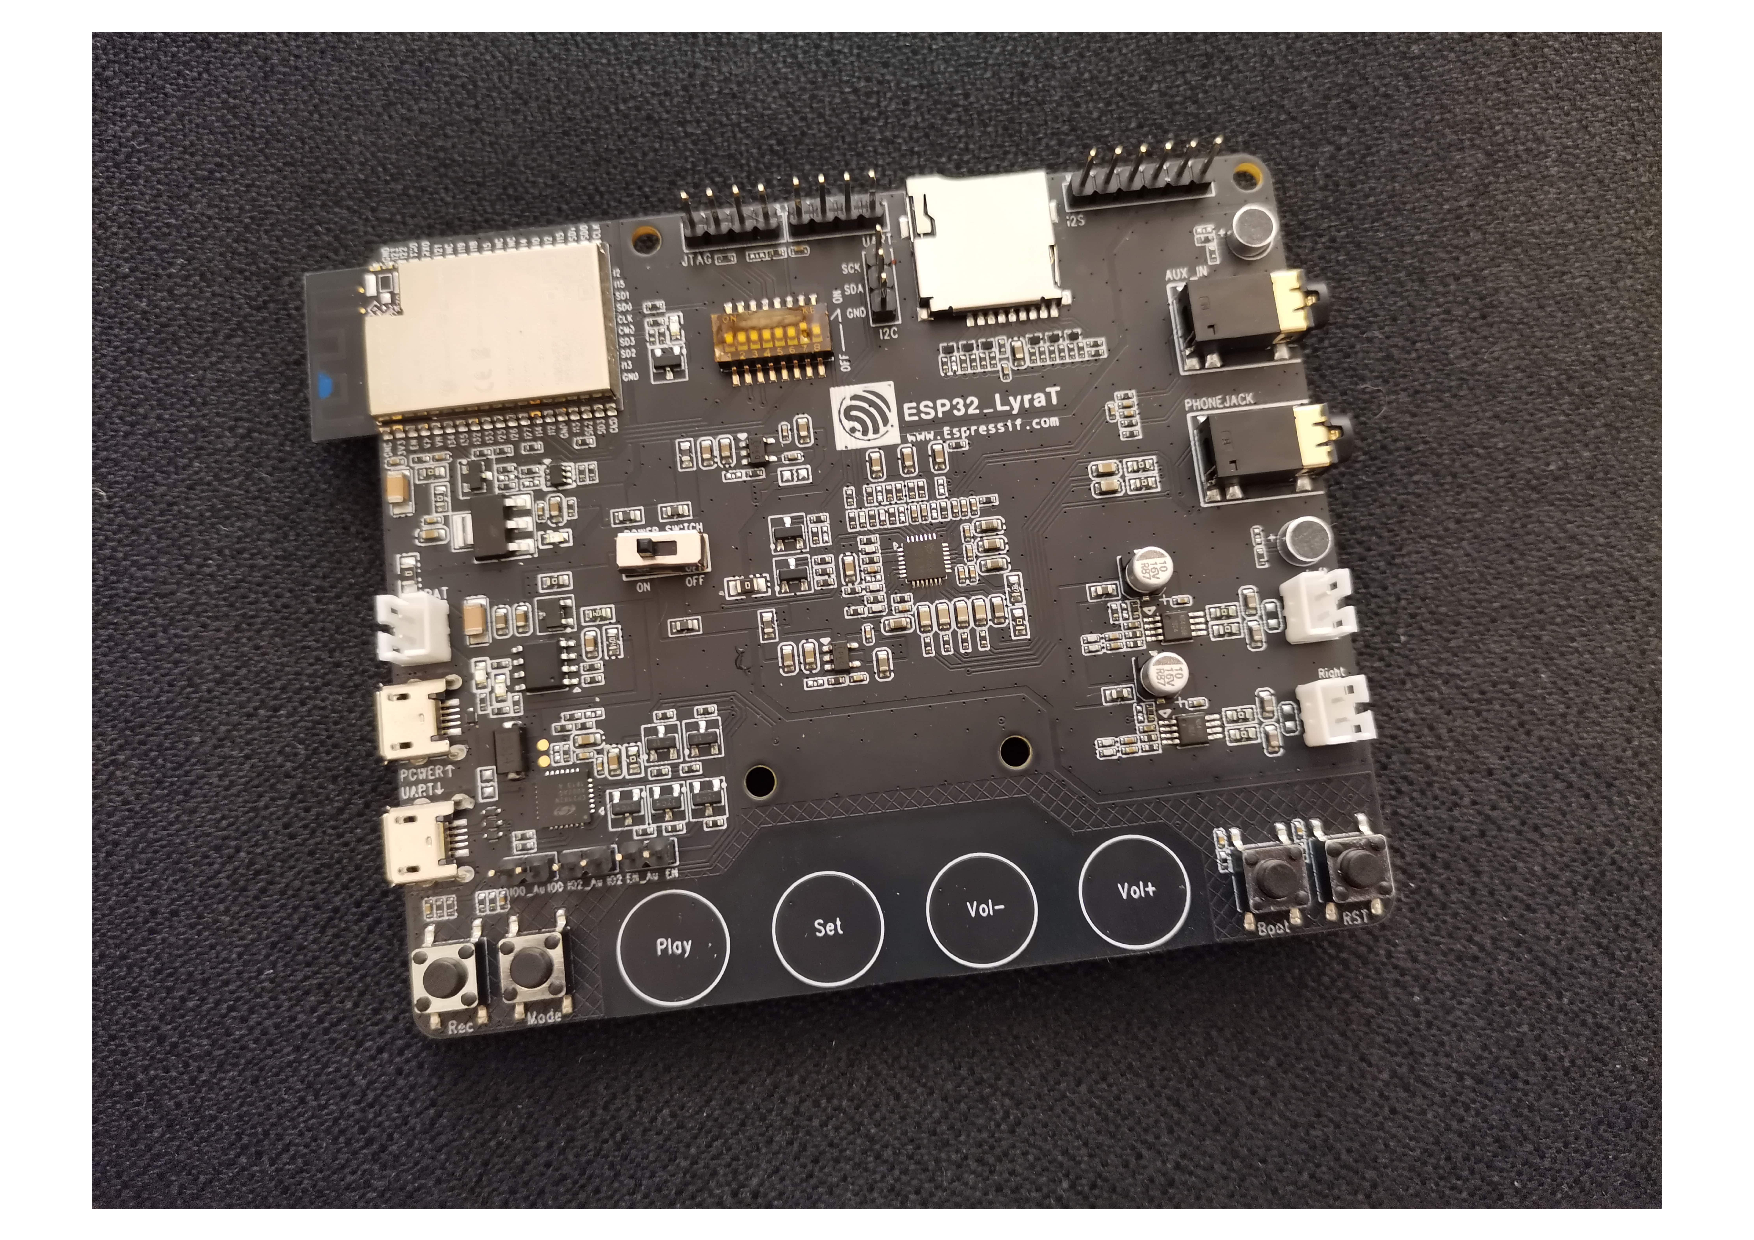
\includegraphics[width=1\linewidth]{images/ESP32-LyraT-1.pdf}
\end{minipage}%
\begin{minipage}{.5\textwidth}
  \centering
  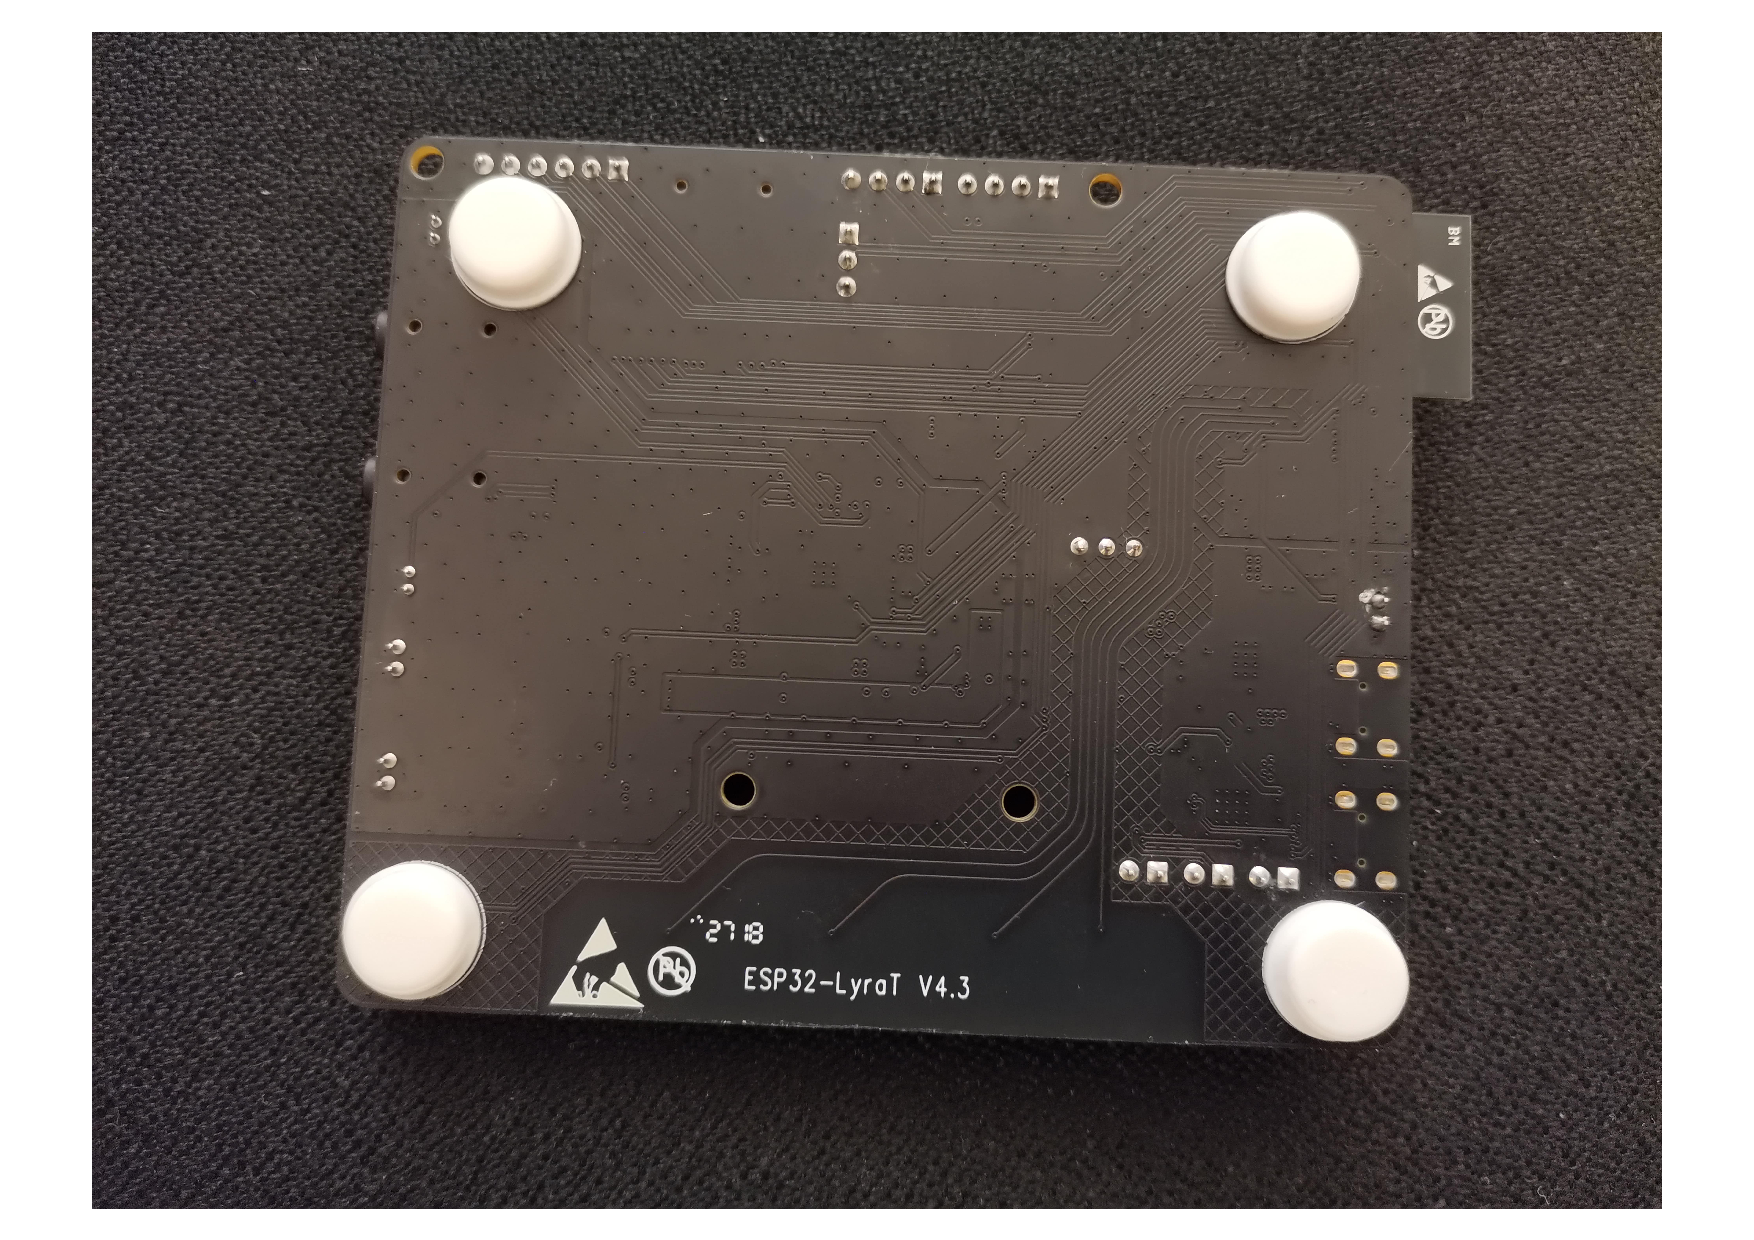
\includegraphics[width=1\linewidth]{images/ESP32-LyraT-2.pdf}
\end{minipage}
\caption{ESP32-LyraT}
\label{esp32-lyrat}
\end{figure}
\fi

It is an audio development board built around ESP32 with additional hardware:
\begin{itemize}
\item	ESP32-WROVER Module
\item	Audio Codec Chip
\item	Dual Microphones on board
\item	Headphone input
\item	2x 3-watt Speaker output
\item	Dual Microphones on board
\item	Dual Auxiliary Input
\item	MicroSD Card slot
\item	Buttons
\item	JTAG
\item	Integrated USB-UART Bridge Chip
\item	Li-ion Battery-Charge Management
\end{itemize}

The main reason for selecting this platform is inbuild external memory of the capacity 8MB. With this size of memory, it should be without any problems to implement selected algorithms. But in reality only 4MB are able to be used in the implementation, more information can be found in section \ref{esp-memory}. Added with excelent documentation at "docs.espressif.com" it was relatively easy to choose this platform for development.

\bigskip
\noindent
The implementations are the same as reference implementations with my adjustments. What I did is that I tried to port them on ESP32 platform.

%%%%%%%%%%%%%%%%%%%
\subsection{Setup of environment}
Fisrt step of development on ESP32 is to set up of environment. This setting I did on Ubuntu 19.10 operating system, starting with downloading of tools:
\begin{lstlisting}[frame=single]
sudo apt-get install git wget libncurses-dev flex bison gperf \
python python-pip python-setuptools python-serial python-click \
python-cryptography python-future python-pyparsing  \
python-pyelftools cmake ninja-build ccache libffi-dev libssl-dev
\end{lstlisting}

\bigskip
\noindent
Add current logged user to group \textit{dialout} because the user needs to get read and write access to the serial port over USB.
\begin{lstlisting}[frame=single]
sudo usermod -a -G dialout $USER
\end{lstlisting}

\bigskip
\noindent
Download software libraries provided by Espressif, Espressif IoT Development Framework (esp-idf), to folder "\$HOME/esp". I used release version 4.1:
\begin{lstlisting}[frame=single]
cd $HOME/esp
git clone -b release/v4.1 --recursive \
https://github.com/espressif/esp-idf.git
\end{lstlisting}
Be \textbf{aware} that all of the setting is related to absolute path "\$HOME/esp". 

\bigskip
\noindent
Install tools used by "esp-idf" to directory "\$HOME/.espressif":
\begin{lstlisting}[frame=single]
cd \$HOME/esp/esp-idf
./install.sh
\end{lstlisting}

\bigskip
\noindent
Last step is to set up environment variables in the terminal where is going to be used "esp-idf":
\begin{lstlisting}[frame=single]
. $HOME/esp/esp-idf/export.sh
\end{lstlisting}
But I added it to file \textit{.bashrc}:
\begin{lstlisting}[frame=single]
echo ". $HOME/esp/esp-idf/export.sh" >> $HOME/.bashrc
\end{lstlisting}
This way it will be added to every new shell session.

\subsubsection{Build \& Load}
To load application to ESP32-LyraT, one must first build the project. For example, copy the project "src/esp/luov" (in the Diploma thesis sources) to "\$HOME/esp/luov". In this folder it is possible to build it:
\begin{lstlisting}[frame=single]
idf.py -n build
\end{lstlisting}
The switch "-n" will stop treat the warrnings as errors.

\bigskip
\noindent
After successful buil,d it is possible to load/flash application to ESP32-LyraT:
\begin{lstlisting}[frame=single]
idf.py -p /dev/ttyUSB0 flash
\end{lstlisting}
The value of the port can be different it depend on to which is ESP32-LyraT connected to.

\bigskip
\noindent
When the loading/flashing starts, it will be waiting for connection from ESP32-LyraT. At that moment hold boot button and press restart button.

\bigskip
\noindent
To check if application is indeed running after loading/flashing, use monitoring system:
\begin{lstlisting}[frame=single]
idf.py -p /dev/ttyUSB0 monitor
\end{lstlisting}
For ESP32-LyraT, when monitoring starts, press restart button.

\bigskip
\noindent
It is possible to combine previous commands together:
\begin{lstlisting}[frame=single]
idf.py -p /dev/ttyUSB0 build flash monitor
\end{lstlisting}

%%%%%%%%%%%%%%%%%%%
\subsubsection{Memory} \label{esp-memory}
Microcontroller ESP32-LyraT has 8MB of external memory (SRAM/SPIRAM). But it is 32-bit processor that means, if external RAM is enabled, only 4MB can be allocated using standard \textit{malloc} calls. To use the region above the 4MB limit, it is possible to use the \textit{himem API}.

\bigskip
\noindent
\textbf{Configuration} - For enabling the external RAM, navigate to "menuconfig $\rightarrow$ Component config $\rightarrow$ ESP32-specific $\rightarrow$ Support for external, SPI-connected RAM $\rightarrow$ SPI RAM config". To access "menuconfig":
\begin{lstlisting}[frame=single]
idf.py menuconfig
\end{lstlisting}

\bigskip
\noindent
\textbf{Stack} - It is possible to change size of the stack for the application. Setting can be found at "menuconfig $\rightarrow$ Component config $\rightarrow$ Common ESP-related $\rightarrow$ Main task stack size".

\bigskip
\noindent
\textbf{Himem} - API which enables access to the remaining memory of external RAM. However this is done through a bankswitching scheme. Configuration can be found at the same place in menuconfig as external RAM.

%%%%%%%%%%%%%%%%%%%
\subsection{Project description}
Base project of esp-idf is composed of the:
\begin{itemize}
\item	build - A folder where the output of build process is stored.
\item	components - A folder which contains subprojects or external projects of the application.
\item	main - A folder which contains source codes of the application. It is also called the \textit{main} component. 
\item	CMakeList.txt - A global setting of the project and starting file for \textit{cmake}. 
\item	sdkconfig - A setting of \textit{menuconfig}.
\item	sdkconfig.default - A default setting of \textit{menuconfig}.
\end{itemize}
But for good convinience I added to this structure a file:
\begin{itemize}
\item	README.md - A file with basic information about build.
\end{itemize}

\noindent
The project can be build by using \textit{make} or \textit{cmake}. For simplicity and recommendation in documentation, also almost every example is written in it, I decided to use \textit{cmake}.

\bigskip
\noindent
Main entry point of application running on ESP32 is function \textit{app\_main}. In provided implementations it can be found in file \textit{main/test.c}.

%%%%%%%%%%%%%%%%%%%
\subsection{LUOV} \label{esp-luov-make}
To make a port of LUOV reference implementation to ESP32, first I needed to create \textit{CMakeList.txt} in folder \textit{main}. This file contains build options for the \textit{main} component.
\begin{lstlisting}[frame=single]
idf_component_register(SRCS INCLUDE_DIRS PRIV_REQUIRES)
\end{lstlisting}
Function is for registering project component to internal build structure of \textit{idf} API.
\begin{itemize}
\item	SRCS  - Files of source codes.
\item	INCLUDE\_DIRS - Paths to header files.
\item	PRIV\_REQUIRES - Components which needs to be build before \textit{main} component and then linked to it.
\end{itemize}

\noindent
It is nessessary to set up path to \textit{idf} compilator header files ortherwise the default, in my case GCC, headers will be used which are incompactible with ESP32.
Last part of this file is block which take care of parsing build flags of project in variable \textit{B\_FLAGS}. 

\bigskip
\noindent
The implementation require component \textit{XKCP} for PRNG. But how it can be seen in the file \textit{components/XKCP/CMakeList.txt} it only request few files from the \textit{XKCP} project. That means it is not necessary to build the whole project but only the requied parts. This way it will reduce the size of the final application. 

\bigskip
\noindent
One of the important required chages is a change of default value for size of stack to 20000B. This size is sufficient to support all of the stack memory allocation. Also it needs to enable the use of external memory. Both of the settings are set in \textit{sdkconfig.default}.

\bigskip
\noindent
The reference implemenation has implementation (file \textit{rng.c}) of random number generator (RNG) from NIST standard. But this RNG require library \textit{OpenSSL} which by default is not part of the \textit{esp-idf}. I found there is a component \textit{esp-wolfssl} which is embedded SSL library and offers a simple API with OpenSSL compatibility layer. Unfortunately when caling initialization function of the \textit{OpenSSL} the ESP32-LyraT will do a segmentation fail. It means that it is not possible to use it.

\bigskip
\noindent
What is possible to do and what I also did, is to change the RNG to hardware RNG of ESP32. But there is condition in which Wi-Fi or Bluetooth needs to be enabled otherwise it can not be considered a true random number generator but only pseudo-random number generator.

\bigskip
\noindent
Implementation can be found in folder \textit{src/esp/luov}. 

\subsubsection{Optimalization}
Because this ported implementation of LOUV is fast and has low memory consumption (see chapter \ref{test-and-disk}), I did not try to make any optimalization attempts. 

\subsubsection{Memory} \label{esp-luov-memory}
To be able measure the allocated memory in ESP32, I implemented memory measurement with the help of \textit{esp-idf} API. Implementation can be found in file \textit{memory\_measurement.c}.

\bigskip
\noindent
This measurement will create new independent task which periodically ask the ESP32 about internal and external memory status. Because the ESP32 is dual-core proccessor, the slowdown by this task should be minimal and this should have minimal influence on signing algorithm. But to by sure there is no slowdown, the speed measurement was taken without this memory measurement.

\bigskip
\noindent
To anable this functionality, the folowing flag needs to be set:
\begin{itemize}
\item	MEM\_MEASUREMENT
\end{itemize}

%%%%%%%%%%%%%%%%%%%
\subsection{Rainbow}
To make a port of Rainbow reference implementation to ESP32, I proceeded in the same way as for the LUOV ESP32 implementation. That means I created \textit{CMakeList.txt} in folder \textit{main} with the same formalities as \textit{CMakeList.txt} for LUOV, see section \ref{esp-luov-make}. The most eye catching difference is set up of different kinds of \textit{malloc}, see section \ref{esp-rb-memory} for more information.

\bigskip
\noindent
The implementation require component \textit{wolfssl} for PRNG. In this case is build the whole \textit{esp-wolfssl} project which is simply added throught \textit{PRIV\_REQUIRES} in \textit{main/CMakeList.txt}. Here is important to mention that Rainbow reference implementation contains two PRNG (see \textit{utils\_prng.c}). One from NIST standard, it is the same RNG as in LUOV reference implementation, and second PRNG which use hash SHA function. Because the RNG form NIST standard was not possible for me to run on ESP32-LyraT, I change it to second PRNG and  I deleted from source codes the implementation of the first.

\bigskip
\noindent
The source codes also require RNG which I changed to hardware RNG of ESP32, it is the same change as in LUOV ESP32 implementation (see \textit{rng.c}).

\bigskip
\noindent
The default value for size of stack I set up to value 5000B. Because this value is sufficient to support all of the Rainbow stack allocation memory. Setting is set up in \textit{sdkconfig.default} with enabled external memory to get access to external 4MB RAM.

\bigskip
\noindent
Implementation can be found in folder \textit{src/esp/rb}. 

\subsubsection{Optimalization}
I did two memory optimalizations of Rainbow implementation for ESP32:
\begin{itemize}
\item	First I found potential big allocation of memory and switch them from stack to heap. Candidates to change were temporary helpful variables of keys (\textit{sk\_t}) in computation of keys from seeds.

\item	Second I created \textit{my\_ESP\_malloc} and \textit{my\_ESP\_free} functions, see \ref{esp-rb-memory}. With these I found that temporary variables (for example \textit{sk\_t* tempQ}) were using lot of memory but in reality only needed a part of the key structure. See commit \textit{"ESP - RB memory reduction in cyclic generation"}, hash \textit{"1609d70c"} for details of optimalization.
\end{itemize}

Witch these two optimalization there was alredy enough memory and I was able to run \textit{\_RAINBOW256\_92\_48\_48} implementation in compressed form. I was also able to run the same implementation in cyclic form but there is same kind of bug and it was making segmentation fault. I am suspecting that it is the same bug 
which causes failure of signature verification.

\subsubsection{Memory} \label{esp-rb-memory}
To be able to better measure the allocated memory in ESP32, there is the same memory measurement implementation as in LUOV ESP32 \ref{esp-luov-memory}, which can be enabled by flag:
\begin{itemize}
\item	MEM\_MEASUREMENT
\end{itemize}

Because I needed better technique for memory allocation on heap, I created my own allocation information table. It is simple small array, I expect small number of allocation at one point at time, which holds imformation of pointer and its size.
It can be enabled by flag:
\begin{itemize}
\item	MY\_ESP\_MALLOC
\end{itemize}
When this flag is set, it will switch all \textit{aligned\_alloc} to \textit{my\_ESP\_malloc} and \textit{free} to \textit{my\_ESP\_free} and every time when there is allocation od deallocation it will print its information.
This information table helped me to identify potential places in source code of RB for memory optimalization. For implementation details see file \textit{malloc.c}.

\bigskip
\noindent
The reference implementation use \textit{aligned\_alloc} function for allocation of memory but ESP32 with toolchain 8.2 which I am using has issue with this function and it is not possible to use for now. That is the reason why I change it to classic \textit{malloc} function.

%%%%%%%%%%%%%%%%%%%%%%%%%%%%%%%%%%%%%%%%%%%%
\newpage
\section{Conventional algorithms}
These selected conventional algorithms were also implemented on microcontroller ESP32-LyraT for the possibility of comparison with LOUV and RB. These two algorithms are one of the most typical and most used in computer for signature schemes, that means there exist very good software implementations with hardware acceleration on ESP32 chip. 

\bigskip
\noindent
Both of the selected algorihms are implemented, using the esp-idf API, in similar way like previous implemetations in this thesis on ESP32. That means their entry point is in file \textit{test.c} which has similar structure to others \textit{test.c} files in previous description. The main difference is in private and public keys which are now in the form of \textit{context} relative to algorithm.

\subsection{RSA}
Test implementation of RSA starts with initialization of context:
\begin{lstlisting}[frame=single]
mbedtls_rsa_context ctx;
mbedtls_rsa_init(&ctx,MBEDTLS_RSA_PKCS_V15,0);
\end{lstlisting}

\noindent
Second step is generation of keypair:
\begin{lstlisting}[frame=single]
mbedtls_rsa_gen_key(&ctx,coap_prng_impl,NULL,KEY_SIZE,EXPONENT);
\end{lstlisting}

\noindent
Generation \textit{hash} of message $m$:
\begin{lstlisting}[frame=single]
mbedtls_sha256(m,message_size,hash,0);
\end{lstlisting}

\noindent
Sign \textit{hash} and put signature to \textit{sm}:
\begin{lstlisting}[frame=single]
mbedtls_rsa_pkcs1_sign(&ctx,coap_prng_impl,NULL,
			MBEDTLS_RSA_PRIVATE,MBEDTLS_MD_SHA256,
			0,hash,sm);
\end{lstlisting}

\noindent
Verify signature \textit{sm} of \textit{hash}:
\begin{lstlisting}[frame=single]
mbedtls_rsa_pkcs1_verify(&ctx,coap_prng_impl,NULL,
			MBEDTLS_RSA_PUBLIC,MBEDTLS_MD_SHA256,
			0,hash,sm);
\end{lstlisting}

\bigskip
\noindent
The implementation can be set with flags:
\begin{itemize}
\item	KEY\_SIZE - Size of public key in bits.
\item 	EXPONENT - Public exponent to use.
\item 	MEM\_MEASUREMENT  - Enable memory measurement.
\end{itemize}

%%%%%%%%%%%%%%%%%%%
\subsection{ECDSA}
Test implementation of ECDSA is very similar to RSA. It starts with initialization of context:
\begin{lstlisting}[frame=single]
mbedtls_ecdsa_context ctx;
mbedtls_ecdsa_init(&ctx);
\end{lstlisting}

\noindent
Second step is generation of keypair:
\begin{lstlisting}[frame=single]
mbedtls_ecdsa_genkey(&ctx,EC_CURVE,coap_prng_impl,NULL);
\end{lstlisting}

\noindent
Generation \textit{hash} of message $m$:
\begin{lstlisting}[frame=single]
mbedtls_sha256(m,message_size,hash,0);
\end{lstlisting}

\noindent
Sign \textit{hash} and put signature to \textit{sm}:
\begin{lstlisting}[frame=single]
mbedtls_ecdsa_write_signature(&ctx,MBEDTLS_MD_SHA256,hash,
			hash_len,sm,&smlen,coap_prng_impl,NULL);
\end{lstlisting}

\noindent
Verify signature \textit{sm} of \textit{hash}:
\begin{lstlisting}[frame=single]
mbedtls_ecdsa_read_signature(&ctx,hash,hash_len,sm,smlen)
\end{lstlisting}

\bigskip
\noindent
The implementation can be set with flags:
\begin{itemize}
\item	EC\_CURVE\_BITS  - Number of bits for eliptic curve.
\item 	MEM\_MEASUREMENT  - Enable memory measurement.
\end{itemize}


%%%%%%%%%%%%%%%%%%%%%%%%%%%%%%%%%%%%%%%%%%%%
%%%%%%%%%%%%%%%%%%%%%%%%%%%%%%%%%%%%%%%%%%%%
\chapter{Testing and discussion} \label{test-and-disk}
\section{PC}
Security cathegories; graphs of times; memory from ref. pdf
\subsection{Time complexity}
\begin{figure}[H]
\centering
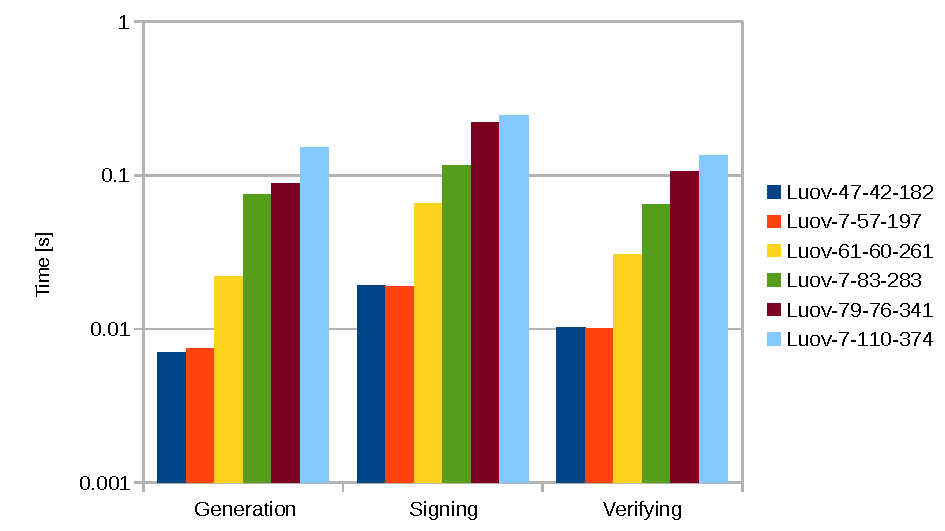
\includegraphics[width=13cm,height=7cm]{images/pc-luov.pdf}
\caption{Porovnání naivních implementací}
\label{pc-luov}
\end{figure}

\begin{figure}[H]
\centering
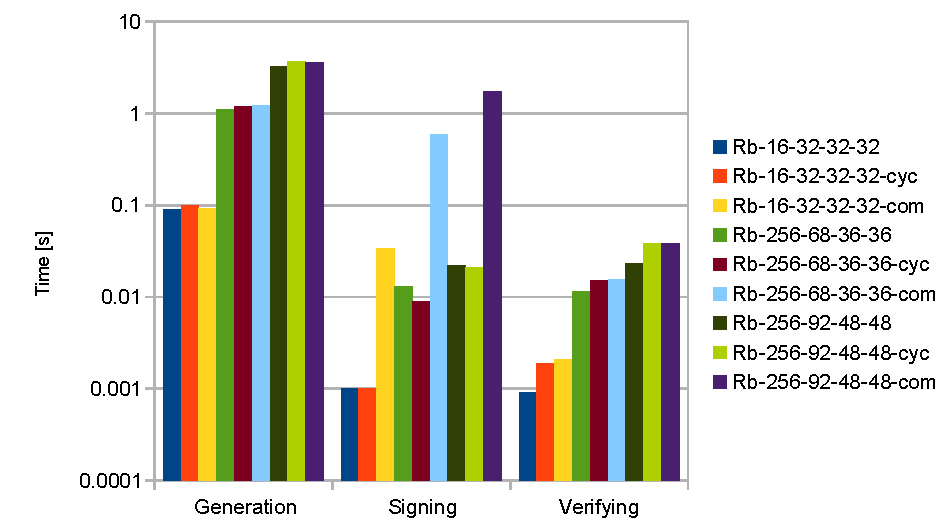
\includegraphics[width=13cm,height=7cm]{images/pc-rb.pdf}
\caption{Porovnání naivních implementací}
\label{pc-rb}
\end{figure}

\begin{figure}[H]
\centering
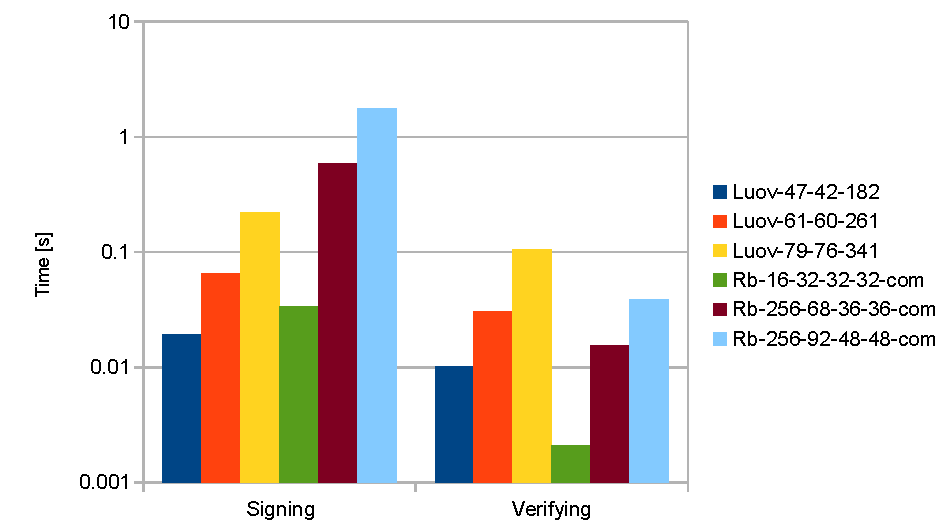
\includegraphics[width=13cm,height=7cm]{images/pc-all.pdf}
\caption{Porovnání naivních implementací}
\label{pc-all}
\end{figure}

%%%%%%%%%%%%%%%%%%%
\subsection{Memory complexity}

%%%%%%%%%%%%%%%%%%%%%%%%%%%%%%%%%%%%%%%%%%%%
\newpage
\section{ESP32}
\subsection{Time complexity}
\begin{figure}[H]
\centering
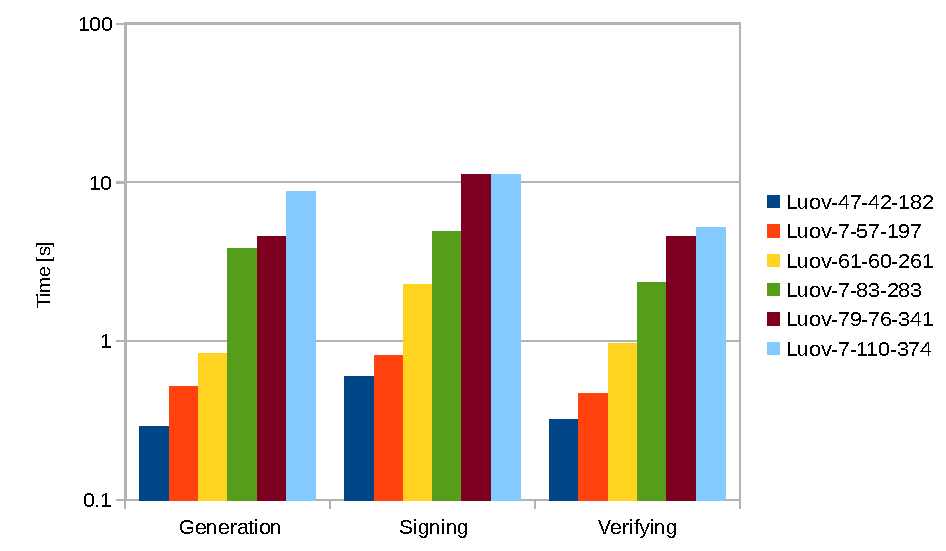
\includegraphics[width=13cm,height=7cm]{images/time-luov.pdf}
\caption{Porovnání naivních implementací}
\label{time-luov}
\end{figure}

\begin{figure}[H]
\centering
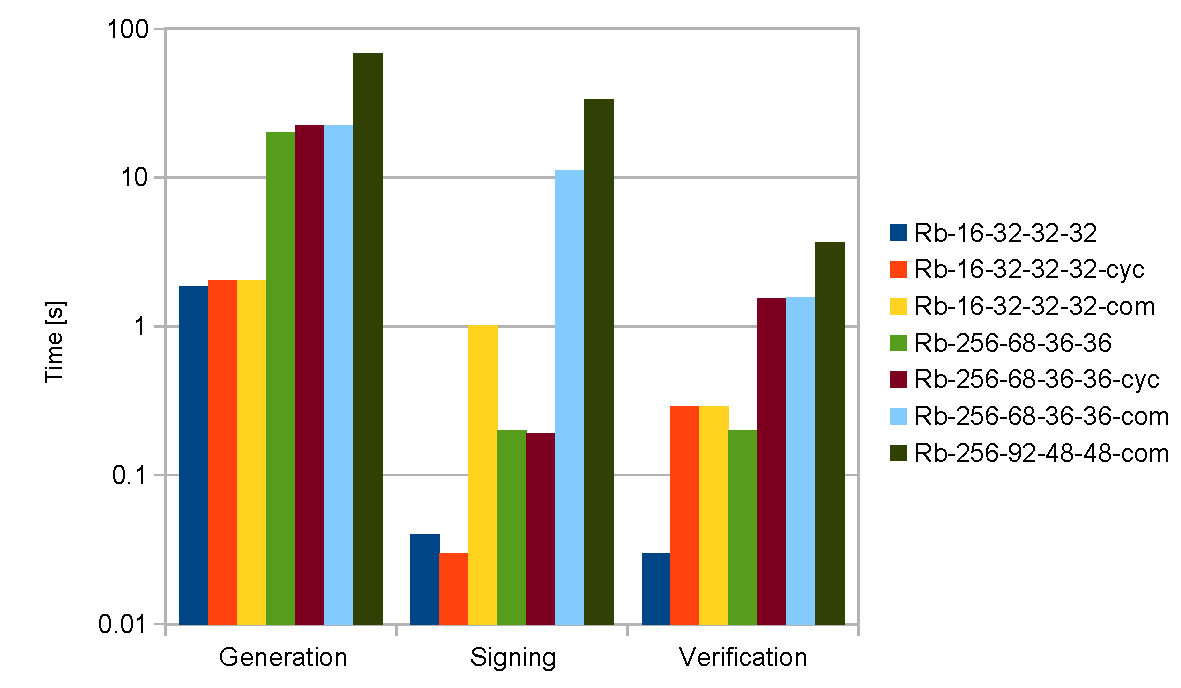
\includegraphics[width=13cm,height=7cm]{images/time-rb.pdf}
\caption{Porovnání naivních implementací}
\label{time-rb}
\end{figure}

\begin{figure}[H]
\centering
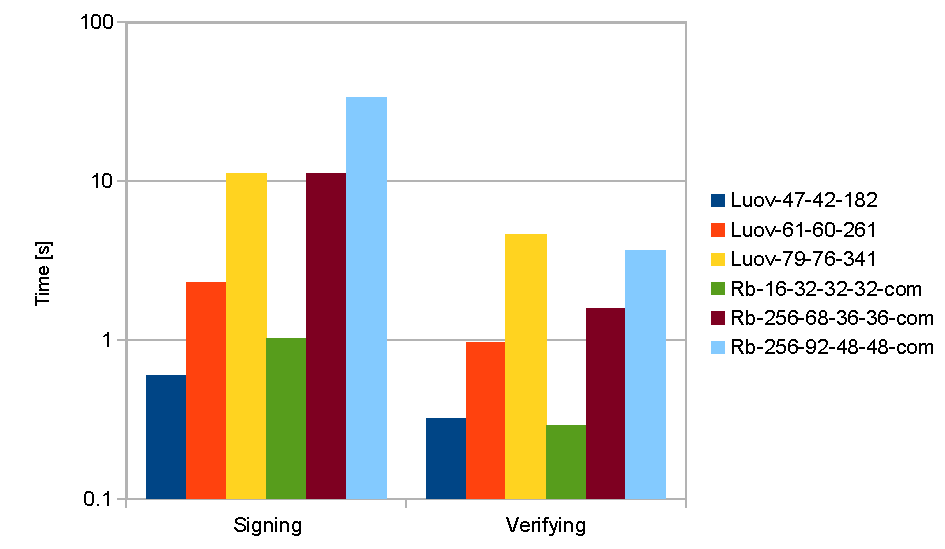
\includegraphics[width=13cm,height=7cm]{images/time-both.pdf}
\caption{Porovnání naivních implementací}
\label{time-both}
\end{figure}

%%%%%%%%%%%%%%%%%%%
\subsection{Memory complexity}
\begin{figure}[H]
\centering
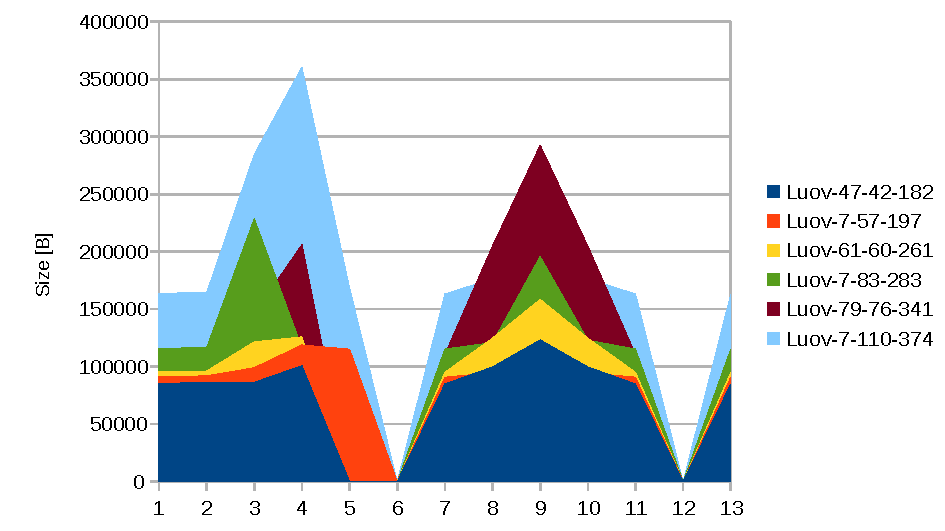
\includegraphics[width=13cm,height=7cm]{images/mem-luov0.pdf}
\caption{Porovnání naivních implementací}
\label{mem-luov0}
\end{figure}

\begin{figure}[H]
\centering
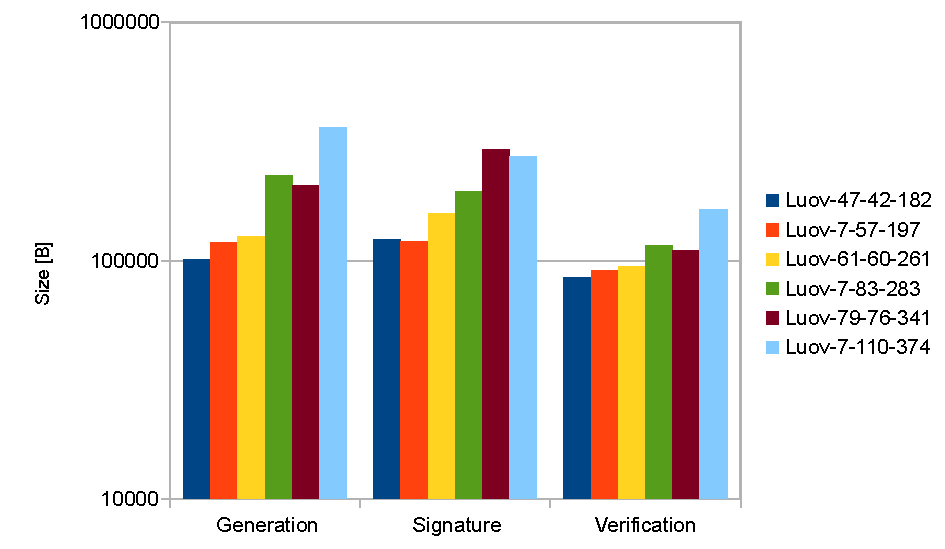
\includegraphics[width=13cm,height=7cm]{images/mem-luov.pdf}
\caption{Porovnání naivních implementací}
\label{mem-luov}
\end{figure}

\begin{figure}[H]
\centering
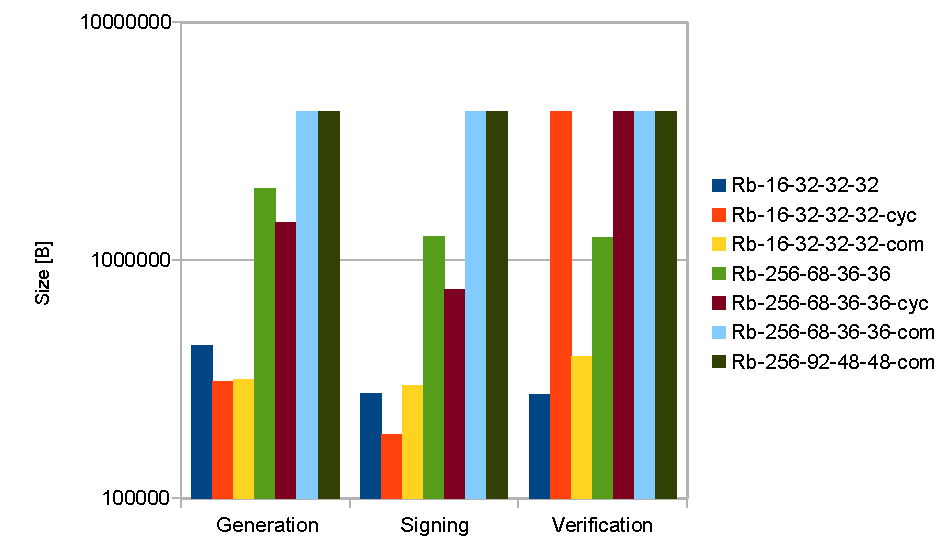
\includegraphics[width=13cm,height=7cm]{images/mem-rb.pdf}
\caption{Porovnání naivních implementací}
\label{mem-rb}
\end{figure}

\begin{figure}[H]
\centering
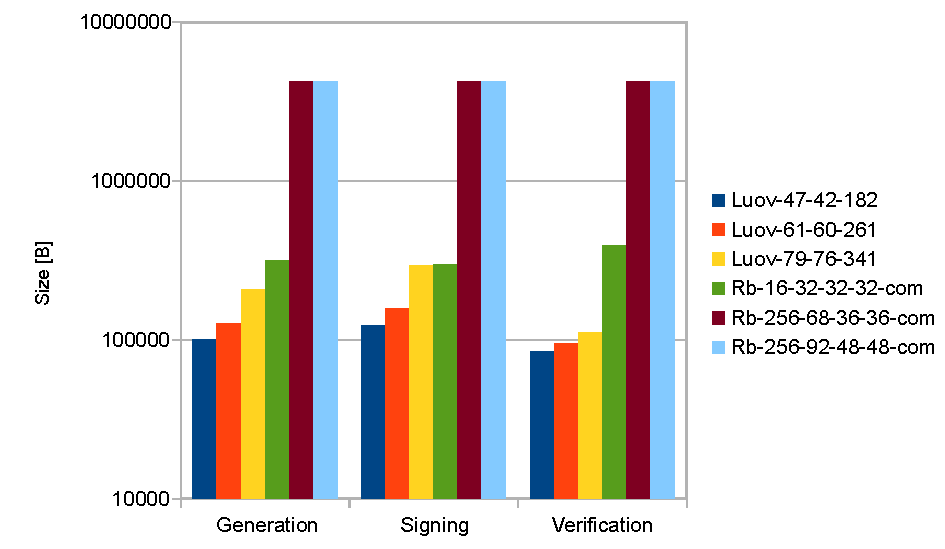
\includegraphics[width=13cm,height=7cm]{images/mem-both.pdf}
\caption{Porovnání naivních implementací}
\label{mem-both}
\end{figure}

\begin{figure}[H]
\centering
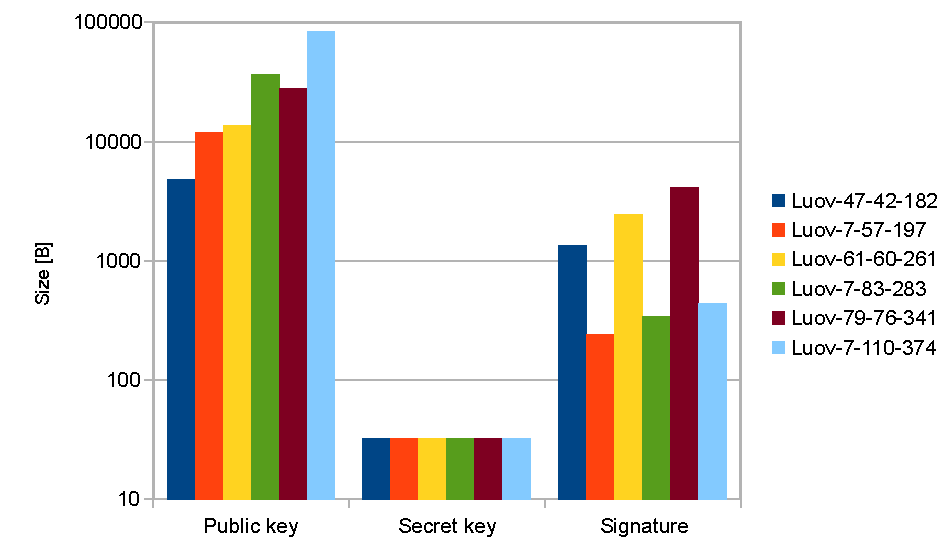
\includegraphics[width=13cm,height=7cm]{images/sign-luov.pdf}
\caption{Porovnání naivních implementací}
\label{sign-luov}
\end{figure}

\begin{figure}[H]
\centering
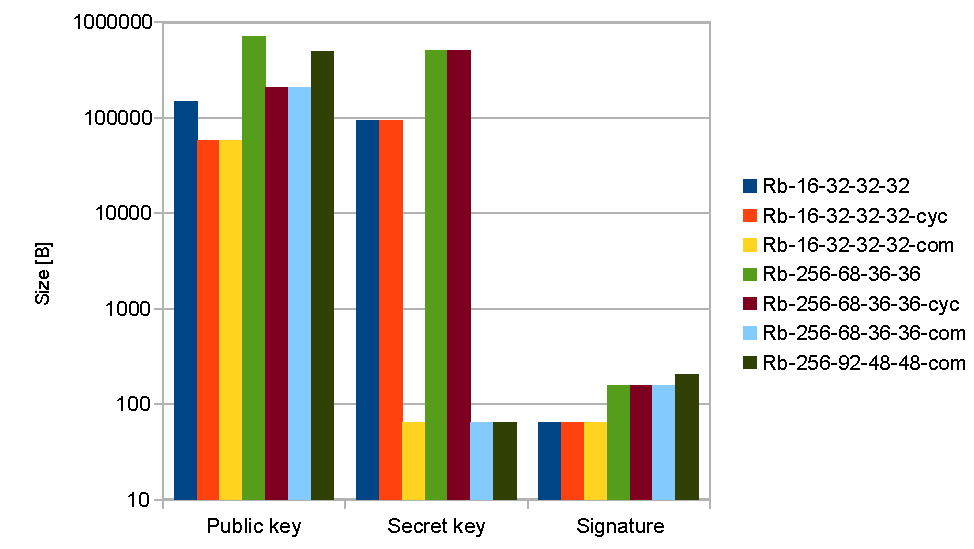
\includegraphics[width=13cm,height=7cm]{images/sign-rb.pdf}
\caption{Porovnání naivních implementací}
\label{sign-rb}
\end{figure}

%%%%%%%%%%%%%%%%%%%%%%%%%%%%%%%%%%%%%%%%%%%%
\newpage
\section{Conventional algorithms}
RSA, ECDSA

\begin{figure}[H]
\centering
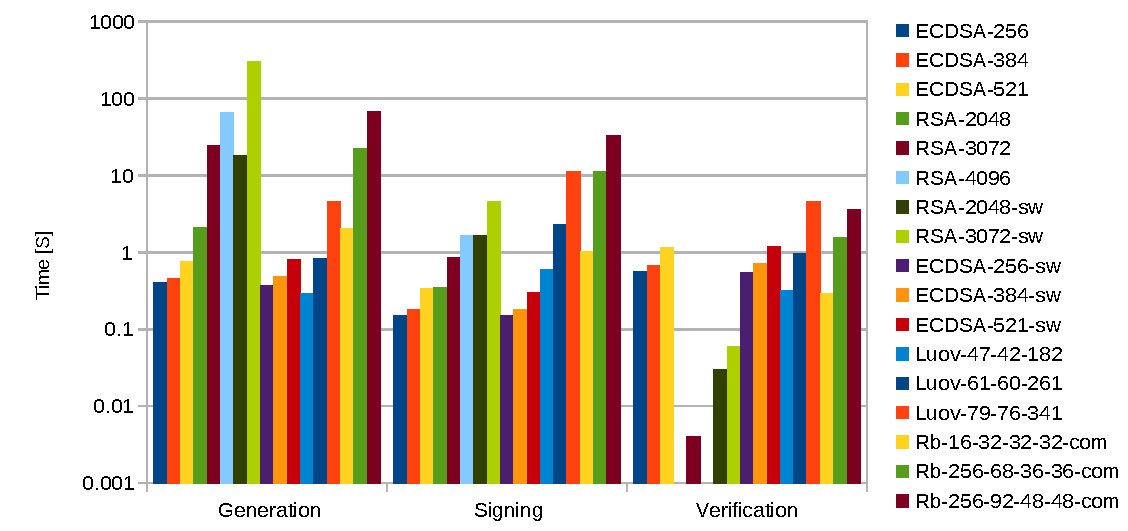
\includegraphics[width=13cm,height=7cm]{images/time-all.pdf}
\caption{Porovnání naivních implementací}
\label{time-all}
\end{figure}

\begin{figure}[H]
\centering
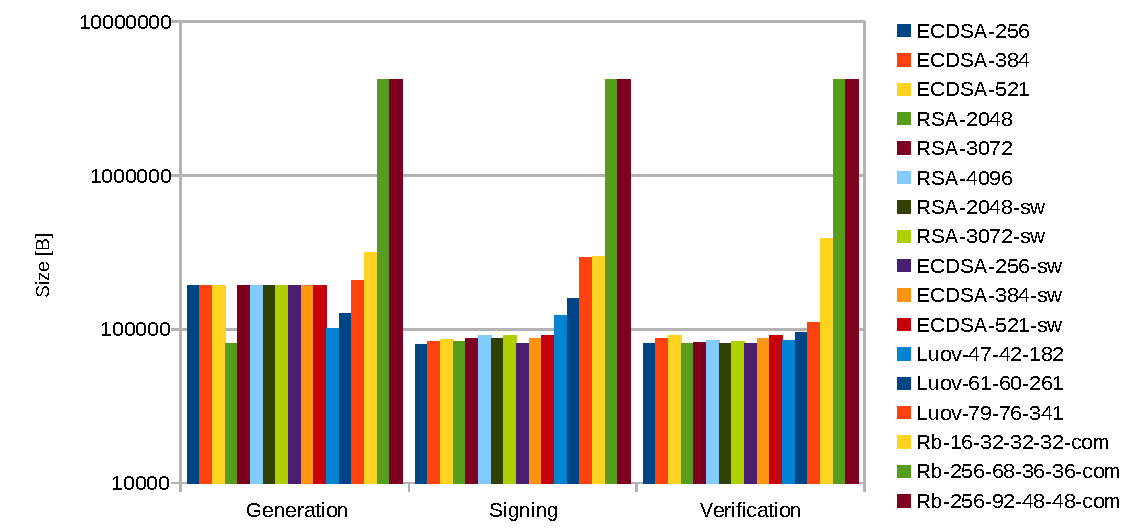
\includegraphics[width=13cm,height=7cm]{images/mem-all.pdf}
\caption{Porovnání naivních implementací}
\label{mem-all}
\end{figure}

%%%%%%%%%%%%%%%%%%%%%%%%%%%%%%%%%%%%%%%%%%%%
%%%%%%%%%%%%%%%%%%%%%%%%%%%%%%%%%%%%%%%%%%%%
\setsecnumdepth{part}
\chapter{Conclusion}
How good I was...; LOUV is much more better...

%%%%%%%%%%%%%%%%%%%%%%%%%%%%%%%%%%%%%%%%%%%%
%%%%%%%%%%%%%%%%%%%%%%%%%%%%%%%%%%%%%%%%%%%%
\bibliographystyle{iso690}
\bibliography{mybibliographyfile}

\begin{thebibliography}{9}
\bibitem{L-CZYP}
CZYPEK, P.: \textit{Implementing Multivariate Quadratic Public Key Signature Schemes on
Embedded Devices.}  Ruhr-Universit\"{a}t Bochum, 2012.

\bibitem{L-PET1}
PETZOLDT, A.: \textit{Multivariate Cryptography Part 1: Basics} [online]. 2017, [cit. 2020-04-1]. At: \url{https://2017.pqcrypto.org/school/slides/1-Basics.pdf}

\bibitem{L-PET2}
PETZOLDT, A.: \textit{Multivariate Cryptography Part 2: UOV and Rainbow} [online]. 2017, [cit. 2020-04-1]. At: \url{https://2017.pqcrypto.org/school/slides/2-UOV+Rainbow.pdf}

\bibitem{L-GEOV}
GEOVANDRO, C.C.F.P.: \textit{Introduction to Multivariate Public Key Cryptography} [online]. 2013, [cit. 2020-04-1]. At: \url{http://www.ic.unicamp.br/ascrypto2013/slides/ascrypto2013_geovandropereira.pdf}

\bibitem{L-MC0}
GOUBIN, L.; PATARIN, J.; YANG, BY.: \textit{Multivariate Cryptography.} In: van Tilborg H.C.A., Jajodia S. \textit{Encyclopedia of Cryptography and Security.} 2011, Springer, Boston, MA

\bibitem{L-MC1}
DING, J.; PETZOLDT, A.: \textit{Current State of Multivariate Cryptography.} In: \textit{IEEE Security \& Privacy.}, vol. 15, no. 4, pp. 28-36, 2017.

\bibitem{L-WIKI1}
\textit{Multivariate cryptography} [online]. 2020, [cit. 2020-04-1]. At: \url{https://en.wikipedia.org/wiki/Multivariate_cryptography}

\bibitem{L-KS98}
KIPNIS, A.; SHAMIR, A.: \textit{Cryptanalysis of the oil and vinegar signature scheme}. In \textit{CRYPTO 1998}, LNCS vol. 1462, pp. 257–266, Springer, 1998.

\bibitem{L-NIST-2ND}
\textit{NIST - Post-Quantum Cryptography, Round 2 Submissions} [online]. 2020, [cit. 2020-04-1]. At: \url{https://csrc.nist.gov/Projects/post-quantum-cryptography/round-2-submissions}

\bibitem{L-EQ-KEYS}
WOLF, CH.; PRENEEL, B.: \textit{Equivalent keys in multivariate quadratic public key systems}. In \textit{Journal of Mathematical Cryptology}, pp. 375–415, 2011.

\bibitem{L-LIFTING}
BEULLENS, W.; PRENEEL, B.: \textit{Field lifting for smaller UOV public keys}. In \textit{Progress
in Cryptology INDOCRYPT 2017: 18th International Conference on Cryptology in India}, Springer, 2017.

\bibitem{L-RB-CYC}
PETZOLDT, A.; BULYGIN, S.; BUCHMANN, J.: \textit{Multivariate
Signature Scheme with a Partially Cyclic Public Key.} In: \textit{INDOCRYPT.} 2010, vol. 6498, pp. 33 - 48. Springer, 2010.

\end{thebibliography}
%%%%%%%%%%%%%%%%%%%%%%%%%%%%%%%%%%%%%%%%%%%%
%%%%%%%%%%%%%%%%%%%%%%%%%%%%%%%%%%%%%%%%%%%%
\setsecnumdepth{all}
\appendix

\chapter{Acronyms}
% \printglossaries
\begin{description}
	\item[ECDSA] Elliptic Curve Digital Signature Algorithm
	\item[IoT] Internet of Things
	\item[LUOV] Lifted Unbalanced Oil and Vinegar
	\item[MC] Multivariate cryptography
	\item[MQ] Multivariate quadratics
	\item[NIST] National Institute of Standards and Technology
	\item[OV] Oil and Vinegar
	\item[PRNG] Pseudo-random number generator
	\item[RNG] Random number generator
	\item[UOV] Unbalanced Oil and Vinegar	
\end{description}


\chapter{Contents of enclosed CD}

%change appropriately

\begin{figure}
	\dirtree{%
		.1 README.md\DTcomment{the file with CD contents description}.
		.1 exe\DTcomment{the directory with executables}.
		.1 src\DTcomment{the directory of source codes}.
		.2 esp\DTcomment{implementation for esp32 platform}.
		.2 mathematica\DTcomment{implementation in Mathematica}.
		.2 offline\DTcomment{offline reference materials}.
		.2 esp\DTcomment{implementation for PC platform}.
		.2 thesis\DTcomment{the directory of \LaTeX{} source codes of the thesis}.
		.1 text\DTcomment{the thesis text directory}.
		.2 thesis.pdf\DTcomment{the thesis text in PDF format}.
	}
\end{figure}

\end{document}
